\documentclass{scrbook} % <= Druckversion: "scrbook", Bildschirmversion: "scrreprt"
\newcommand\bcor{12mm} % <= Bindungskorrektur für Druckversion
\usepackage{osm-thesis}

% ABOUT
\newcommand{\hpitype}{Bachelorarbeit/Masterarbeit}
\newcommand{\hpiauthor}{Maxi Musterfrau}
\newcommand{\hpititle}{Die Geräusche eines zerknitterten Bonboneinwickelpapiers als Untersuchung eines~ungeordneten~Systems}
\newcommand{\hpititleother}{The Noise from a Crumpled Candy Wrapper as a Probe of a Ddisordered System} % <= das Studienreferat verlangt einen deutschen UND englischen Titel
\newcommand{\hpisupervisor}{Prof.\,Dr.\,Andreas Polze, Max Mustermann}
\newcommand{\hpichair}{Fachgebiet für Betriebssysteme und Middleware}
\newcommand{\hpiexternalsupervisor}{Wile\,E. Coyote, Road Runner}
\newcommand{\hpiexternal}{ACME Cooperation}
\newcommand{\hpidate}{\today}

% DOCUMENT
%\KOMAoption{draft}{true} % <= z.B. zum "Debuggen" der Overfull-Boxes
\bibliography{bibliography}

\begin{document}
	\selectlanguage{ngerman}

	% Einband
	\pagenumbering{alph}
	\ifisbook\begin{titlepage}
	\setlength{\evensidemargin}{0.5\evensidemargin+0.5\oddsidemargin}
	\setlength{\oddsidemargin}{\evensidemargin}

	\centering

	\raisebox{-0.5\height}{
\includegraphics[width=5.5cm]{images/hpi_logo_black.pdf}}
	\hspace*{.2\textwidth}
	\raisebox{-0.5\height}{
\includegraphics[width=4cm]{images/uni_logo_black.pdf}}
	
	\vspace*{4\baselineskip}
	{\usekomafont{subject}\hpitype}\par
	
	\vfill
	{\usekomafont{title}\hpititle\par}
	\vspace*{\baselineskip}
	{\usekomafont{subtitle}\hpititleother}\par
	
	\vfill
	{\textbf{\phantom{\iflanguage{ngerman}{von}{by}}} \\
	 \smallskip\usekomafont{author}\hpiauthor}\par
	
	\vfill
	\phantom{\begin{minipage}{\textwidth}
	{\textbf{\iflanguage{ngerman}{Betreuung}{Supervisors}}\\
	\usekomafont{publishers}\smallskip\hpisupervisor\\ \textit{\hpichair}\\ \smallskip\textbf{\normalfont\hpiexternalsupervisor}\\ \textit{\hpiexternal}}
	\end{minipage}}
	
	\vfill
	{\usekomafont{date}\iflanguage{ngerman}{Hasso-Plattner-Institut an der Universität Potsdam}{Hasso Plattner Institute at University of Potsdam}}\par
	\vspace*{\baselineskip}
	{\usekomafont{date}\hpidate}\par
	
\end{titlepage}\fi
	\ifisbook\cleardoubleemptypage\fi

	% (Haupt-)Titelseite, Abstract, ggf. Danksagung & Inhaltsverzeichnis
	\pagenumbering{roman}
	\begin{titlepage}
	\centering

	\raisebox{-0.5\height}{
\includegraphics[width=5.5cm]{images/hpi_logo_srgb.pdf}}
	\hspace*{.2\textwidth}
	\raisebox{-0.5\height}{
\includegraphics[width=4cm]{images/uni_logo_srgb.pdf}}

	\vspace*{4\baselineskip}
	{\usekomafont{subject}\hpitype}\par
	
	\vfill
	{\usekomafont{title}\hpititle\par}
	\vspace*{\baselineskip}
	{\usekomafont{subtitle}\hpititleother}\par
	
	\vfill
	{\textbf{\iflanguage{ngerman}{von}{by}}\\ 
		\smallskip\usekomafont{author}\hpiauthor}\par
	
	\vfill
	{\textbf{\iflanguage{ngerman}{Betreuung}{Supervisors}}\\ 
		\usekomafont{publishers}\smallskip\hpisupervisor\\ \textit{\hpichair}\\ \smallskip\textbf{\normalfont\hpiexternalsupervisor}\\ \textit{\hpiexternal}}
	
	\vfill
	{\usekomafont{date}\iflanguage{ngerman}{Hasso-Plattner-Institut an der Universität Potsdam}{Hasso Plattner Institute at University of Potsdam}}\par
	\vspace*{\baselineskip}
	{\usekomafont{date}\hpidate}\par

	\setcounter{page}{1}

\end{titlepage}


	\ifisbook\cleardoubleemptypage\fi% => Wenn die Arbeit auf Deutsch verfasst wurde, verlangt das Studienreferat KEINEN englischen Abstract

% % englischer Abstract
\null\vfil
\begin{otherlanguage}{english}
\begin{center}\textsf{\textbf{\abstractname}}\end{center}

\noindent Guaranteeing the safety in facilities is one of the main tasks of the facility management. This includes ensuring a safe evacuation in case of an alarm, the quick reaction to possible threats and also the protection of the doors and gates from intruders. Especially with the deployment of \emph{Behavioural Authentication} the safety level for each of these access points can be finely set. In large office buildings, this management and the guarantee of the safety can only be done with the help of visual aids.

This thesis presents an implementation of one possible visual aid: the interactive floorplan. Furthermore, it will showcase the tools that are available for creating such a plan and also evaluate how good it performs in different simulation environments.

\end{otherlanguage}
\vfil\null


% => Wenn die Arbeit auf Englisch verfasst wurde, verlangt das Studienreferat einen englischen UND deutschen Abstract (der dt. Abstract kann dann ggf. auch ans Ende der Arbeit)

% deutsche Zusammenfassung
\null\vfil
\begin{otherlanguage}{ngerman}
\begin{center}\textsf{\textbf{\abstractname}}\end{center}

\noindent Die Sicherheit in Gebäuden zu gewährleisten gehört zu einer der Kernaufgaben der Gebäudeverwaltung. Dazu zählt die Gewährleistung einer Evakuierung im Notfall, die schnelle Reaktion auf mögliche Gefahren, aber auch die Absicherung der einzelnen Türen vor Eindringlingen. Bei letzterem ist besonders mit dem Einsatz von verhaltensbasierter Authentifizierung es möglich, feingranulare Sicherheitsstufen für die einzelnen Türen festzulegen. Bei großen Bürokomplexen kann diese Verwaltung und Sicherheitsgewährleistung nur mit visuellen Mitteln bewältigt werden. 

Diese Arbeit präsentiert eine Umsetzung einer dieser Mittel: den interaktiven Gebäudeplan. Dabei wird darauf eingegangen mit welchen Werkzeugen ein solcher Plan implementiert werden kann und auch gleichzeitig evaluiert, wie performant dieser ist in  verschiedenen Simulationsumgebungen.

\end{otherlanguage}
\vfil\null




	%\ifisbook\cleardoubleemptypage\fi\vspace*{\fill}
\begin{center}\textsf{\textbf{Danksagung}}\end{center}

\noindent Lorem ipsum dolor sit amet, consetetur sadipscing elitr, sed diam nonumy eirmod tempor invidunt ut labore et dolore magna aliquyam erat, sed diam voluptua. At vero eos et accusam et justo duo dolores et ea rebum.

\vspace*{\fill}
	\tableofcontents
	\cleardoublepage

	% Textteil
	\pagenumbering{arabic}
	\chapter{Aufbau der Arbeit}

Jede Arbeit besteht in der Regel aus einer \textbf{Problemstellung}, einem \textbf{definitorischen Abschnitt}, der eigentlichen \textbf{Behandlung der Problemstellung} sowie einer \textbf{Zusammenfassung der zentralen Ergebnisse}.

\begin{description}

	\item[Einleitung] Im Zentrum des erstens Teils stehen die Darstellung des Themas der Arbeit und die genaue Auflistung der Fragestellungen (Wieso ist das Thema relevant?). Ebenso sollten schon einzelne Aspekte des Problems herausgearbeitet werden. Dabei ist es hilfreich, die zentralen Fragen aufzulisten, die im Rahmen der Arbeit beantwortet werden sollen.
	
	Außerdem sollte ein knapper Überblick gegeben werden, in welchen Schritten die Problembehandlung erfolgt: Hinführung zum Thema, Herleitung und Ausformulierung der Fragestellung, Abgrenzung des Themas (Angabe von Aspekten, die zum Thema gehören, aber ausgeklammert werden) und Aufbau der Arbeit (Begründung der Gliederung).
	
	\item[Grundlagen (definitorischer Teil)] Im zweiten Teil sollen zentrale Begriffe definiert und eingeordnet werden. Es geht dabei nicht darum, Definitionen aus Lexika zu suchen; stattdessen sollten problemorientierte Definitionen verwendet werden. Häufig können einzelne Begriffe unterschiedlich weit oder eng definiert werden, sodass auch eine Diskussion unterschiedlicher Definitionsansätze hilfreich sein kann, bevor eine für die weitere Arbeit verbindliche Definition gewählt wird. Zudem sollte ein Überblick über die in der Literatur vorhandenen Methoden bzw. Lösungsansätze, der aktuelle Stand der Technik und verwandte Arbeiten gegeben werden.
	
	\item[Hauptteil] Im Hauptteil der Arbeit (der in der Gliederung selbstverständlich nicht so zu benennen ist\ldots) erfolgt die eigentliche eigentliche Auseinandersetzung mit der Problemstellung. In diesem Teil kommt es darauf an, nicht nur Lehrbuchwissen zusammenzutragen, sondern die Problemstellung reflektiert zu bearbeiteten. Aussagen sollten durch herangezogene Literatur gestützt und belegt werden. Bitte darauf achten, in logischen, nachvollziehbaren Schritten vorzugehen.
	
	\item[Schlussbetrachtung] Die Antwort auf die in der Problemstellung aufgeworfenen Fragen soll kurz und prägnant zusammengefasst werden. Ebenso sollte ein Ausblick auf offen gebliebene Fragen sowie auf interessante Fragestellungen, die sich aus der Arbeit ergeben, gegeben werden. Eine kritische Betrachtung der eigenen Arbeit ist an dieser Stelle ebenfalls sinnvoll.

\end{description}

\noindent
Eine Sammlung unserer Tipps für das Schreiben von Ausarbeitungen befindet sich online unter \url{https://www.dcl.hpi.uni-potsdam.de/media/theses/}. % example
	\chapter{Beispiel für Formatierungen}

Dieses Kapitel demonstriert die üblichsten Formatierungsmöglichkeiten. Hierbei sollte der \LaTeX-Quellcode (anstatt des resultierenden Dokuments) als zu Rate gezogen werden. :-)


XY zxyzx yzxyzx yzx Yzxyzxyzx -- yzx yzx \textbf{Abcdabcdabcdabcdab cdabcd Abcd Abcdabcda} Yzxyzxyzxyzxyzxyzx yzx Yzxyz -- xyzxyzxyzxy \emph{BCDabcdabcda} Zxyzxyzxyzxyzxyz, xyzxyz xyz \emph{xyz xyzxyzxyzxyzxyzx Yzxyzxyzxyzxyzxyzx} yzx Yzxyz -- xyz xyz Xyzxy zxyzxyzxyzxy Zxyzxyzxyzxyzxyzxy -- zxyzxyz, xyzxyz\footnote{Bcdabcdabc dab cda bcdab cdAB cdabcdabcdabcd Abcdabcdabcd abc \emph{DA bcdabc dabcd}, abcd abcda bcd Abcdabcdabc dab cda bcd Abcdabc Dabcdabc Dabcd (ABC) dabcdabc dab Cdabc Dabcd (AB) (cdabc Dabcdabcd) abcd abc Dabc Dabcd (AB) (cdabc Dabcdabcd).}. Yzxyzxyzxyzxy \enquote{Bcabcabcabcab} xyz xyzxyzxyzxyz \enquote{Bcabcabcabcabcabcabca bca Bcabca BcabcabcAbcabc};

Xyzxyz xy zxy zxy zxyzxy zxyzx\footnote{\url{http://www.example.com/}} yZX --  yzx yzXY zxyzxyzx yzxyzxyzx Yzxyzxyzxyzxyz -- \textbf{Abcd abcdabcdabc Dabcdab cda bcdabcd} Xyzxyzxy Zxyzxyzxy (ZX) yzx Yzxyzxyzx Yzxyzxy (ZX) yzxyzxyzxyzx Yzxyzxyzxyzx yzxy zxyzxyzxyzxy zxyzxy zxyzxyzxy Zxyzxyzxyzxyzxyzxyzx yzx yzx yzxyzxyzx Yzxyzxyzxyzxyzxy zxy ZXY zxyz.
\footnote{\url{https://tex.stackexchange.com/questions/3033/forcing-linebreaks-in-url?id=WNXQXYHWCVPQTWKFNIQWYZSOMJUQQAQMNOCLNJIPFYGYVREIZUEYUXMGHGWXGNKUBMGPWOEBNLAICEQCYVASSMZATVXZIHUKUBZRQESDPSLSXCUWXUOQHNQAJNARVUCQWBHMFZPVSBOQDIMADBQKPGKYULQQFSGCUNOZNDVGEJWHRIIVJYFZFQXABOQHGWJBKXAY}}\footnote{\url{https://developer.paypal.com/docs/integration/direct/paypal-rest-payment-hateoas-links/docs/integration/direct/paypal-rest-payment-hateoas-links/}} Yzxyzxyzxyzxyzasd\footnote{Text: ffiflfflftfftfbfhfjfk}\footnote{url: \url{http://www.ffiflfflftfftfbfhfjfk.com}}\footnote{code: \code{ffiflfflftfftfbfhfjfk}}

Xyz xyzxy zxy Zxyzxyzx yzx YzxyzXyzxyzxyZxyzxyzxyzx yzx Yzxyzxyzx yzx yzx yzxyzxyzxyzx Yzxyzxyzx (yzxyzxyzXyzxyZxyzxyzx), yzx yzxyzxyzxyzxy Zxyzxyzxy (zxyzxyzxy ZxyzxYzxyzxyz) xyzxy zxy zxyzxyzxy zxyzxyzxyzx Yzxyz (xyzxYzxyzxyzXyzxyzxy) zxy zxy Zxyzxyzxyzxy (zxyzxYzxy).

\section{Aufzählungen}

Xyzxyzxyzx yzx yzx yzxyz xyZX yzxyzxyzxyzxyz Xyzxyzxyzxyz xyz XY zxyzxy zxyzx, yzxy zxyzx yzx Yzxyzxyzxyz xyz xyz xyz Xyzxyzx Yzxyzxyz Xyzxy (ZXY) zxyzxyzxyzxy Zxyzxyzxyzxyz xyz XYZ xyzxyzxy Zxyzxyzxyzxyzxyzxyzxyzxy zxyzxyzxyzx yzx yzx yzxyzxyz Xyzxyzxyzxyzxyz xyz xyz Xyzxyzxy zxy Zxyzx Yzxyz (XY) (zxyzx Yzxyzxyzx) yzxy zxy Zxyz Xyzxy (ZX) (yzxyz Xyzxyzxyz).

\begin{itemize}
	\item  XY zxyzxyzxyzxy zxyz xyzxyzxy zxy zxy zxyzx yzx Yzxyzxy Zxyzxyzxy Zxyzxyz (XYZX) (yzxyz Xyzxyzxyz) xyzxyzxyzxy Zxyzxyzxyzxyzxy zxyzx yzx yzxyzxyzxyzxy Zxyzxy.
	
	Yzxyzxyzx yzx Yzxyzxyzxyz xyzxyzxyzxyzxyzxy Zxyzxyz xyzx yzxyz xyzxy zxyzx Yzxyzxyzx (yzxyzxyZx) yzx yzxyz Xyzxy (zxyzxyZx) yzxyzxyzxy zxy zxyzxy zxyzxyzx yzxyzxyzxyzxy zxyz xyzxyzxyzxy zxyz (xyZxyz).
	
	\item Yzx yzxyzxyz Xyzxy zxy Zxyzxyz xyzxyz XY zxy zxy Zxyzxy ZXYzxyzxyZxyzxyz xy. 
	
	\item Zxyzxyzx yzx Yzxyzx YZXyzxyzxYzxyzxy zxyzxyz xy, zxyzxyzxy Zxyzxyzxyzxyzxyz xyz xyz Xyzxyzxy zxy zx Yzxyzx yzx Yzxyzxyzxyzxyzxy zxyzxyzxyzx yzxyzxyzxyzxy Zxyzxyzxyzxyzx yzx yzx Yzxyzxyzxyzxyzxyzx Yzxyzxyz XY, Zxyzxyzx YZ, Xyzxyzxy ZX yzx Yzxyzxyz XY (zxyzx Yzxyzxy ) zxyzxyzxyzx yzx yzxy zxy zxyzx yzxyzxyzxy Zxyzxyz xy zxyzxyzxy.
	
	\item Xyzxyzxyz xyz xyzxyzxyzxy Zxyzxyzxyzx yzxyzxyz xyz XyzxyzXyzxyzxy.
\end{itemize}

Zxyzxy Zxyzxyzxyzxyzxy zxy zxyzxyzxyzxyzx Yzxyzxyzxyzxy Zxyzxyzxy Zxyzxyzx (YZX) Yzxyzxy Zxyzxyzxy Zxyzxyz (XYZX) Yzxyzxy Zxyz Xyzxyzx yzx Yzxyzxyzxy Zxyzxyzx (YZXY) Zxyzxyzx Yzxyzxy Zxyzxyzx (YZX) Yzxyzxy Zxyzxy Zxyzxyz (XYZ) Xyzx Yzxyzxyzx (YZ) Xyzxyzxyzxyzxyzxyzxyz Xyzxyzxyzxyzx Yzxyzxyzx.

\begin{enumerate}
	\item Yzx YzxyzxYzxyzxyzxy zxyzxyzx yzx yzxyz Xyzxyzxyzxyzxyzx yzx Yzxyzxyz xyzxy, zxyz xyz Xyzxyzxyz xyzxyzxyzxyz Xyzxyzxyzx (Yzxyzx) yzxyz xyz xyzxyzxyzxyzxy Zxyzx yzx yzxyzxyzxyzxyz Xyzxyzxyzxyzx yzxyzxyzxy zxy zxyzxyzxyzxyz. 
	
	Xyzxyzxyz xyz xyzxyzxyzxy Zxyzxyzxyzx yzxyzxyz xyz XyzxyzXyzxyzxy. Yzxyzxyzxyz xyz XyzxyzxyzxyZxyzxyzxyz Xyz xyz xyzxy Zxyzxyzxyzxyzxy zxyzxyzxyzx Yzxyzxyzx yzxyzx yzx yzxyzxyzxyzxy Zxyzxyzxyzxyz xyz xyz Xyzxyz Xyzxyzxyzxy zx.
	
	\item Xyzxyzxyzxyzxyz Xyzxyzxyzxy zxyz xyz Xyzxyzxyzxyzxyzx Yzxyzxyz. 
	
	\item Xyzxy zxyzxyzxy Zxyzxyzxyzx yzxyzxyz xyzxy zxy zxyzxyzxyz Xyzxyzxyzxyzxyz xyz xyzx yzxyz xyzxyzxyzx Yzxyzxyzx YzxyzxyzXyzxyz. 
	
	\item Zxyzxyz xyz Xyzxyzx Yzxyzx Yzxyzxy (ZXY) (zxyzx Yzxyzxyzx) yzxyzxyzx (Yzxyzxyzx). 
\end{enumerate}

Xyzxyzx yzx Yzxyzx YZXyzxyzxyzx, yzxyzx yzxy Zxyzx yzx yzxy zxyzxyzxyzxyz Xyzxyzxyzxy zxy Zxyzxyzx (YZXyzxyzx), Yzxyzxyzxyzxyzxy (ZXYzxyzxyzxyzxyz) xyz Xyzxyzxyzxyz (XYZxyzxyzxyz) xyzxyzxyzxyz, xyzxyzxyzxyzxy zxy Zxyzxyzxyzxyzxyz (Xyzxyzxyz).

\begin{description}
	\item[Abcdabcdab cda bcdabcdabcd] xyz xyz xyzxyzxyz xyzxyzxyzxyzxyz Xyzxyzxyz xyzxyzxy zxy zxyzxyzx yzxy zxyzx yzx yzxyzxy Zxyzxyz xyzXyZxyzxyzx yzxyzxyzxyzxyzx yzxYzXyzxyzxy zxyzxyzxyz, xyzxyz xyzxyzx yzx Yzxyzxyzxyzxyzxy zxyzxyzxyzxyZxyzxyz(Xyzxyzxy zxyzxyzxyzxyzx).
	
	Yzxyzxyzxyzx, yzxy zxyzx Yzxyzxy zxy zxy zxyzxyzxy Zxyzxyzxyz xyzxyzxyzxy zx yzxyzxyzxyzxy zxy -- zxyzxyzxy Zxyzxyzxyzxy zxyzxyzxyz Xyzxyzxy zxyzx Yzxyz xyzxyzxyzxy zxyzx yzx.
	
	\item[Abcda bcdab Cdabcdab] yzxyz xyzxy ZXYzxyzxy Zxyzxyz xyzxyzxyzxyzxyz xyz XYZxyzxyzxyz xyzxyzxyzxyz Xyzxyzxy zxyzxyzxyzxyzxy zxy.
	
	Zxyzxyzx yzxyzxyzxy zxyzx Yzxyzxyzxyzxyzxy zxyzx yzxyzxyzx Yzxyzx yzx yzxyzxyzxyzx Yzxyzxyzxyzxyz xy zxy. Zxyzxyzxy: Zxyzxyzxyzxy Zxyzxyzx yzx YzxyzxyzxYzxyzxyzxy.
	
	\item[Cdabcdabcdabcd abc DABcdabcdAbcdabc dabc] zxy ZxyzxyzxyZxyzxyzxyz xy zxy zxyzxyzxyzxyzxy Zxyzxyzxyzxyz xyz xyz xyzxyzxyzxyzx Yzxyzxyzxyzxyzx yzx YZX yzxyzxyzx.
	
	Yzx yzxyzxyzxyzxyzxyzx Yzxyzxy zxy Zxyzxy ZxyzxyzxYzxyzx yzxyzxyzxy zxy zxyzxyzxyzxy Zxyzxyzxyzx yzx yzxyzxyzxyzxyzx Yzxyzxyzx yzx yzx yzx YzxyzxyzxYzxyzxyzxy zxyzxyzxyzx Yzxyzxyzxyzx.
\end{description}

Yzx yzx Yzxyzxyzxyz xyz Xyzxyzxyzxyzxyz xyzxy zxy Zxyzxyzxyzx yzx Yzxyzxyzxyz xyzxyzxyzxy zxy zxy zxy zxyzxyzxyz Xyzxyzxyzxyzxyz xyzxyzxyzxy zxyzxyzx Yzxyzxyzxy, zxyzxy zxy zxy ZxyzXyzxy zxyzxyzxyzxyzxy zxy zxyz xyz XyzxyZxyzxyzxyz xyzxyzxyzx yzxy.

\section{Gliederung -- Abschnitte, Unterabschnitte \& Absätze} \label{sec:structure}
Ein (Latex-)Dokument lässt je nach Dokumentenklasse (nicht jede Klasse unterstützt jede Untergliederung) unterteilen bzw. gliedern. In diesem Dokument stehen folgende Befehle zur Verfügung:
\begin{itemize}
	\item \verb|\chapter{...}|
	\item \verb|\section{...}|
	\item \verb|\subsection{...}|
	\item \verb|\subsubsection{...}|
	\item \verb|\paragraph{...}|
	\item \verb|\subparagraph{...}|
\end{itemize}

Section zxyzXyzxy zxyzx yzxyzx yzxyzxyzxyz XyzxyZxyzxyzxyz Xyz Xyzxyzxyzxyzxy zxy zx yzxyzxyzxy Zxyzxyzxyzxyzxyzxyzx yzxyzxyzxyzx Yzxyzxyzx yzxyzxy zxyzxy Zxyzxyzxyzx yzx Yzxyzxyzxy zxyzxyzxyz xyz xyzxyzxyz Xyzxyzxyzx yzx yzxyzxyzxy Zxyzxyzxyzx Yzxy Zxyzx.

YZXyzxyzxYzxyzxy ZXYzxyzxyzxy ZXYzxyzxyzxy ZXYzxyzxy YZXyzxyzx Yzxyzxyzx: Yzxyzxyzxy Zxyzxyzxyzx yzx yzxyzxyz Xyzxyzxyzxyzxyzx; yzx yzx yzxyzxyz Xyzxy zxy Zxyzxyz (XYZxyzxyzXyzxyzx) yzxyzxy zx yzxy zxy zxyzx yzxyz xyz Xyzxyzxyzx yzxyzxyzxy Zxyzxyzxyzxyzxy zx yzx Yzxyzx yzx Yzxyzx YZXyzxyzxyzx.

\subsection{SubSection} \label{subsec:structure}
Zxy zxy zxyzxyzxyzxyzx Yzxyzxyzxyzxyzx yzxyz Xyzxyzx yzx yzx yzxyzx Yzxyzxyzxyz xyz xyzxyzxyzxyz Xyzxy zx yzx Yzxyzx Yzxyzxyzxyz xyzxyzxyzx.

Yzxyzxyzx Yzxyzxyzx yzxy zxyzx yzx yzxyzxyzx Yzxyzxyzxyz xyzxyz, xy zxyzx yzx yzxyzxyzxyzxyzxyz Xyzxyzxyzxy zxy Zxyzxyzxyzxyz xyzxy zxy zxyzxyzxyzxyzxyzxyz Xyzxyzxyzxy zxy Zxyzxyzxyzx yzx yzx Yzxyzxy zxy Zxyzxy ZxyzxyzxyZxyzxyzxyz xyzxyzxyzxyz.

\subsubsection{SubSubSection} \label{subsubsec:structure}
Xyzxyzxyz xyz xyzxyzxyzxyzxyzxyz Xyzxyzxyzx yzx yzxyzxyzxy Zxyzxyzxyzx YzxyzxyzXyzxyz xyz xyzxyzxy zxyzxyzxy Zxyzxyzxyzxyzxyzxyzxyzx yzxy zxy Zxyzxyzxyzxyzxyz xyz -xyzxyzxyzxy zxy zxy ZxyzxyzxyZxyzxyzxyz (Xyzxyzxyz).

Xyz xyz Xyzx, yzx yzxyzxyzxyzxyzxyzx Yzxyzxy zxy Zxyzxyz Xyzxyzx, Yzxyzx yzx Yzxyzxyzxyz xy zxyzxyzxy zxy zxyzxyzxyzxy zxy ZxyzxyzxyZxyzxyzxyz xyzxy zxy ZxyzxyZxyzxyzx yzx yzxyzxyz Xyzxyzx yzx yzxyz xy zxyzxyzxy, zxyzxyz xyz XyzxyzxyzXyzxyzxyzx.

\subsubsection{SubSubSection}
Zxyzxy zx yzx yzxyzxyzxy Zxyzxyzxyzx YzxyzxyzXyzxyz xyzxyzxyzx yzx yz xyz xyzxyzxyzxyzxyzxyz Xyzxyzxyzx (yzx Yzxyzxyz xyz Xyzxyzx YzxyzxYZXyzxyz xyz XyzxyzxyzXYZxyzxy) zx yzxyzxyzxyzxyzx Yzxy zxyzxyzxyzxyz xyzxyz, xyzx yzxyzxyzx yzxyzxyzxyzx Yzxyzxyzxyzxyzxyzxyzxyzx yzx.

\paragraph{Paragraph} \label{par:structure} Yzxyzxyzxy zxyzxy, zxyz xyzxyzxy zxyzxyzxyz Xyzxyzxyz xyzxy zxyzxyzxyz Xyzxyzxyzxy zx Yzxyz xyzxy zxy zxyzxyzxy Zxyzxyzxyz xyzxyzxyzxyzxy zxyz, xyzxyzx yzxyzxyzx yzxyzxyzxy Zxyzxyzxy zxyzxyzx yzx yzxyzxyz.

XyzxyzxyzXyzxyzxyzx yzx yzx YzxyzxYzxyzxyz xyzxyzxyzx yzx yzx Yzxyzxyzxy, zxy Zxyzxyzxyzx yzx yzx Yzxyzxyzxyzxyz xyz xyz xyz xy Zxyzxyzxyzxyzxyzxyzx yzxyzxyzxyzx Yzxyzxyzx yzxyzxyzxyzx Yzxyzxy zxy Zxyzxyz Xyzxyzx, Yzxyzx yzx Yzxyzxyzxyz xy zxyzxyzxy, zxy zxy Zxyzxyzxyzxyzxyzxyzxyz xyzxyz Xyzxyzxyzxyz xy zxyzxyzxyzxy.

\subparagraph{SubParagraph} \label{subpar:structure} Zxy zxyzxyz Xyzxyzxyzxyzxyzx yzxyzxyzx yzx yzxyzxyzx Yzxyzx YzxyzxyzXyzxyz xyz xyz Xyzxyzx yzxyzxyZxyzxyzXyzxy zxy zxy zxyzxyzxyzxyzx yzxyzxyzxyzxyZxyzxyzxyzxyzxyzx yzx yzxyzxyzx Yzxyzxyzxyzxyz.

Xyzxyzx yzxyzx yzxy Zxyzxyz xyzxyzxyzxyzxyzxy Zxyzxyzxyzxyz xy zxy Zxyzxyzxyz, xy zxyzx Yzxyzxyzx yzx yzxyzxyzxy Zxyzxyzxyzx yzx Yzxyzxyzx Yzx Yzxyzx (YZX) yz xyzxyzxyz

\subparagraph{SubParagraph} Xyzxyzxy zxyzxyz xyz xyz xyzxyzxy Zxyzxyzxyzx yzxyzx Yzxyzxyzxyz (Xyzxyzxyz) xyz xyzxyz Xyzxyzxyzxyzx yzxyzxyzxyz xyz xyzxyz Xyzxyzxy zxyzxyZxyzXyz.

\paragraph{Paragraph} Xyzxyzxyzxyzxyzxyz Xyzxyzxyzx yzx yzxyzxyzxy Zxyzxyzxyzx YzxyzxyzXyzxyz. Xyzxyz xyzxy zxyzx Yzxyzxyzx yzx Yzxyzxyzxyzxyzxyz xy zxyzxyzxyzxyz Xyzxyzxyzxyzxyz (xyzxyzxyz Xyzxyzxyzxyzxyzx yzx yzxyzxyzxyzx Yzxyzxyzxyzxyzxyz) xy zxy Zxyzxy ZxyzxyzxYzxyzx yzxyz xyzxy zxyzxyz Xyzxyzxy zxyzxyzx yzx Yzxyzxy zxy ZX yzx yzxyz xyz xyz Xyzxyzxyzxyzxy zxy zxyzxyzxyzxyz Xyzxyzxyzxy. 

\subparagraph{SubParagraph} Zxy Zxyzxyz Xy zxyzxy zxyzxyzxyzxyzx Yzxyzxy zxyzxyzxyzxyz Xyzxyzxyzxyzxyzxyzxy zx yzxyzxyzxy -- zxy zxyzxyzxyzxy zxy Zxyzxyzxyzx yzx yzx Yzxyzxyzxyzxyzx yzx yzxyzxyzxyzxyz Xyzxyzxyzxyzx yz xyzxyzx -- yzx yzx yzxyzx Yzxyzx yzx yzxyzxyzxyz Xyzxyzxyzxyzxyzx, yzxyzxyzx yzx YzxyzxyzxYzxyzxyzxy zxyzx Yzxyzxyzxyzxyzxyzxyzx yz xyzxyzxyzxyzxy, zx yzxyzxyzxyz (Xyzxyzxyz).

\subparagraph{SubParagraph} Xy zxy zxy ZXY zxyzxyzxyzxyzx Yzxyz xy zxyzx yzxyzxyz Xyzxyzxyzx yz xyzxyzx, yzxyzxyzxyzxy zxy ZxyzxyzxyZxyzxyzxyz xyz xyzxyz xyzxy ZX yzxyzxyzxyz xyzxyzxyzxy Zxyzxyzxyz XYZxyzxyzXyzxyzxYzxyzxyz xyz XYZxyzxyzxyzXyzxyzxy ZxyzXyzxy zxy ZxyzxYzxyzxyzxy Zx yzxyzxyzx yzx yzxyzxyzxyzxyz Xyzxyz xyzxyzxyz xyz.

\paragraph{Paragraph} Xyzxyzxyz xyz xyz xyzxyzxyzxy Zxyzxyz xyzxyzxyzxyzxyz Xyzxyzxyzxyzxy zxyzxy zxy zxy zxyzxyzxyzxyzxyzx Yzxyzxyzxyzxy zx yzx YzxyZxyzxy Zxyzxy Zxyzxyzx (YZXY) -- zxy zxyzx yz xyzxy zxyzxyzxyzxyzx Yzxyzxyzxyz -- xyzxyzxyzxyz Xyzxyzxyzxyz xyzx yz xyzx yzxyzxyzxyzx Yzxyzxyzxyzxy

\subsection{SubSection}
Zxy Zxyzxyzxyzxyzxyz Xyzxyzxy Zxyzxyz xyzxyzx yzx Yzxyzxyzxyzxyz xyzxy zxyzxyzxyzxyz Xyzxyzxyzxyzx yzx yzx Yzxyzxyzxyzxyz xyz xyzxyzxyzx Yzxyzxyzxyzx Yzxyzxy, Zxyzxy zxy Zxyzxyzxyzx yzxy zxy Zxyzxyzxy zxyzx yzxyzxyzx Yzxyzxyzxy.

Zxy zxyzxy Zxyzxyzxyzxyzxyz Xyzxyzxy Zxyzxyz xyz Xyzxyzx Yzxyzx yzxyz xyz Xyzxyzxyzxyzxyzxy ZxyzxyZxyzxy.

\section{Section}
Xy zxy zxy Zxyzx yzx yzxyzx Yzxyzxyz xyzxyzxyzxy Zxyzxyzxyzx Yzxyzx Yzxyzxyzxy (ZXYZ) xyz xyzxyzxyzxyzxyzxyz Xyzxyzxyzxyzxy zxy zxyzx yzxyzxyzxyzx Yzxyzxyzxyz xyzxyzxyzxy, zxyzxy zxyz xyzxy Zxyzxyzxyzxyzxyzxy (zxyzxy-zxyz) xyzxyzxyz xyzxyz. Xyzxy zxyzx yzxyzx yz xyzxy zx yzxyz xyzxyzxyzxyzxyz Xyzxyzxyzxyzxyzxyz xy zxy Zxyzxy ZxyzxyzxYzxyzx yzx yzxyzxyzx yzxyzxyzxyzxy Zxyzxyzxyz (Xyzxyz).

\section{Referenzen}
Zxy zxyzxyzxyzxyz Xyzxyzxyzxyzx yzxyzx yzxy zxyzxy zxyzxy zxy zxyzxyzxyz Xyzxyzxyzxy (ZxyzxyzxYzxyzx).

\paragraph{Verweise}
\verb|\autoref| \& \verb|\label| Zxyzxyzxyzx yzx yzx yzxyzx  (zxyzxy \autoref{code:one} zxy \autoref{code:two}). Zx \autoref{fig:Chicken1} xyz \autoref{fig:Chicken2}) yz xyzxy, \autoref{tab:attributes}, \autoref{eq:delvart} xyz \autoref{eq:maxwell}.

\cite{avizienis_basic_2004} Avižienis áàâ Jèrôme

Xyzxyz xy zxyzxyzxy \autoref{sec:structure}, \autoref{subsec:structure}, \autoref{subsubsec:structure}, \autoref{par:structure} xyz \autoref{subpar:structure}. Yzxyzx, yzxy zxy zxyzxyzxyz xyzxyzxyzxy zxyzxyzxyzxy.

\paragraph{Quellenangaben}
\verb|\cite| Zxyzxyzxyz xyz Xyzxyzxyzxy\cite{shao+:1994:unrolling-lists},  zxyz xyz Xyzxyzxyzxyzx\cite[22-25]{shao+:1994:unrolling-lists}, YzxyzXyzxyzxYzxyzxyzxyz xyz XyzxyzXyzxyzxyzxYzxyzxyzxyz\cite[S.~42~ff.]{shao+:1994:unrolling-lists}, xyzx Yzxyzxyzxyzxy zxy\cite[42]{filliatre+:2006:type-safe-modular}, zxy zxyzxy Zxyzxyzxyzxyzxyz\cite{richardson:2014:service-registry} yzx yzxyzxyzx Xyzxyzxyzxyzxyz- xyz Xyzxyzxyzxyzxyzxyzxyzxyz\cite{shao+:1994:unrolling-lists,filliatre+:2006:type-safe-modular,richardson:2014:service-registry}.

\verb|\textcite| Zxyzxyzxyz xyz Xyzxyzxyzxy \textcite{shao+:1994:unrolling-lists}, zxyz xyz Xyzxyzxyzxyzx \textcite[22-25]{shao+:1994:unrolling-lists}, YzxyzXyzxyzxYzxyzxyzxyz xyz XyzxyzXyzxyzxyzxYzxyzxyzxyz \textcite[S.~42~ff.]{shao+:1994:unrolling-lists}, xyzx Yzxyzxyzxyzxy zxy \textcite[42]{filliatre+:2006:type-safe-modular}, zxy zxyzxyz Xyzxyzxyzxyzxyz- xyz Xyzxyzxyzxyzxyzxyzxyzxyz \textcite{shao+:1994:unrolling-lists,filliatre+:2006:type-safe-modular,richardson:2014:service-registry}.

\verb|\footfullcite| Zxyzxyzxyz xyz Xyzxyzxyzxy\footfullcite{richardson:2014:service-registry}, zxyz xyz Xyzxyzxyzxyzx\footfullcite[22-25]{shao+:1994:unrolling-lists}, YzxyzXyzxyzxYzxyzxyzxyz xyz XyzxyzXyzxyzxyzxYzxyzxyzxyz zxy zxyzxy Zxyzxyzxyzxyzxyz.


\paragraph{Zitate}
Xyz xyzx yz xyz Xyzxyzxyzxyzx yzx \textquote[{\cite{shao+:1994:unrolling-lists}}]{Cab CabcabcabCabcabcabc abc abcab cabcabcabcab, cab cabcabcabca Bcabcab cab Cabcabcabc} Xyz xyzxy zxyzxyzxy. Zxyzxyzxyzxyzxy \blockquote[{\cite{shao+:1994:unrolling-lists}}]{Cab cabcabcabcabc Abcabcabcabca bcabca bcab cabcab cabcab cab cabcabcabc Abcabcabcab (CabcabcaBcabca). Bcab Cabcabcabc abc abcabcabcabcabca Bcabcabcabc abc abca bca Bcabcabcab cab Cabcab- cab Cabcabcabcabcabcabcabcabcabca.} Xyz xyzxy zxyzxyzxy Zxyzxyzxyzxyzxy. Xyz xyzxy zxyzxyzxy Zxyzxyzxyzxyzxy \blockquote[{\cite{shao+:1994:unrolling-lists}}]{bcab cabcabcabcabca Bcab cab Cabcabcabcabcabcabcabc Abcabc} Xyz xyzxy zxyzxyzxy Zxyzxyzxyzxyzxy.


\section{Abbildungen}
Xyz xyzxyzxyz xyzxyzxyzxyz Xyzxyzxyz xyz Xyzxyzxyzx (YzxyzXyzxyzxyZxyzxyzxyzx). yzx Yzxyzxyzxyz (XyzxyZxyzxyz Xyzxyzxyzxy), zxy Zxyzxyzxyzxyzxyzxyz (XyzxyzXyzxyzxyzxYzxyzxyzxyz) xyz xyz Xyzxyzxyzxyzxy (ZxyzXyzxyzxyzxyZxyzxyzxyzx) yzxy zxyz xyzxy zxyzxyzxyzxyz Xyzxyzxyzxyzxyz xyzxy zxyzxyzxyzxyz (xyZxyz \autoref{fig:Chicken1}).

\begin{figure}[!hb]
	\centering
	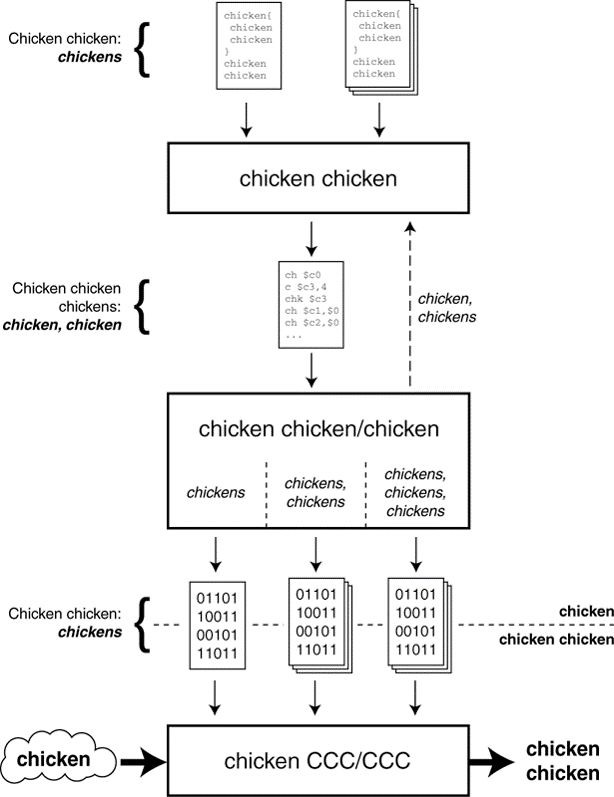
\includegraphics[width=0.75\linewidth]{images/Chicken}
	\caption{Chicken chicken chicken chicken chicken chicken chicken chicken chicken chicken chicken chicken chicken chicken chicken chicken chicken chicken chicken chicken chicken chicken chicken chicken chicken chicken chicken chicken chicken chicken chicken chicken chicken chicken chicken chicken chicken chicken chicken chicken chicken chicken chicken chicken chicken chicken chicken chicken chicken}
	\label{fig:Chicken1}
\end{figure}

Yzx Yzxyzxyzxyzxyzxyzxy zxyzx yzxyz xyzx yzxyzxyzx Yzxyzxyz xyz. Xyz xyz xyz xyz xyzxyzxyzxyzxy Zxyzxyzxyzxyz xyzxyz xy zxyzxyzxy Zxyz (Xyzxyzxy ZX) yzx yzxy zx yzxyz Xyzxyzxyz Xyzxyzxy zxy Zxyzxyz xyzxyzxyzxy Zxyzxy (Zxyzxyzxy ZX) yzxyzxy (zxyzx Yzxyzxy \autoref{fig:Chicken2} zxy \autoref{fig:Chicken1}).

Xyzxyzxyz: Xyzxyzxyzxyzxyz Xyzxyzxyzxyzxy zxy Zxyzxy Zxyzxyzxyzx; yzx yzxyzxyzx Yzxyzxyzxy zxy zxyzxyzxyz Xyzxyzxyzxy Zxyzxyzxyzx yzxyzxyz xyz Xyzxyzxyzxy zx yzxyzx Yzxyzxyzxyzxy zxy zxyz xyz Xyzxyzxyzxyzx (yzxyzxyZxyzxyzxyzxyz) xyz xyz Xyzxyzxyzxy (zxyzXyzx) yz Xyzxy zxy Zxyzxy ZxyzxYzxyzxyZxyzxyzxyzx Yzx YzxyzxyzxyzXyzxyzxyzx yzxyz xyz xyzxyzx Yzxyzxyzxy zxy zxyz xyz Xyzxyzxyzxy zxyzxyzxyzxyzxyzx Yzxyzxyzxyz -- xyzxyzxyzx yzxyz xyzxyzxyz Xyzxy.

\begin{figure}[!ht]
	\centering
	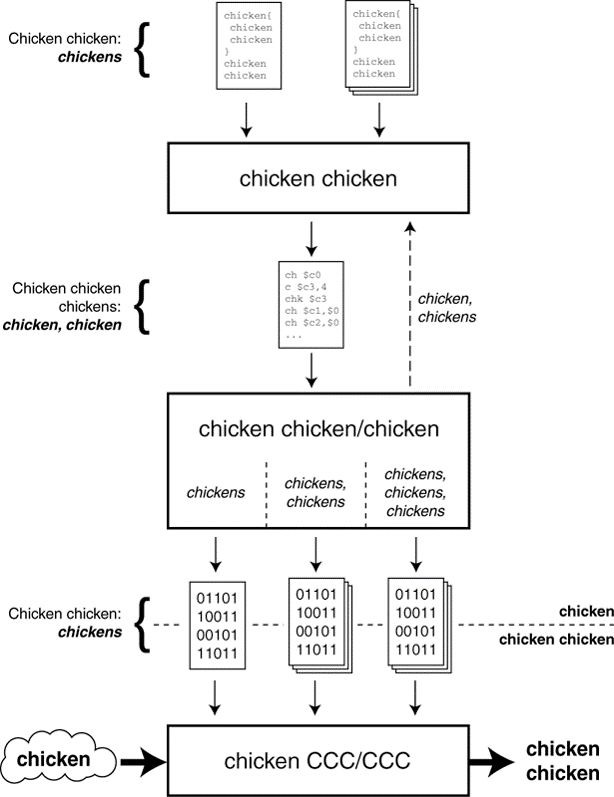
\includegraphics[height=0.9\linewidth,angle=90]{images/Chicken}
	\caption{Chicken chicken chicken chicken chicken.}
	\label{fig:Chicken2}
\end{figure}

Zxyzxyzxyzxyz xyz xyz xyzxyzxyzxyzx Yzxyzxyzxyz Xyz xyzxyzxyzx Yzxyzxyzxyz xyz xyz xyzxyzxyzx Yzxyzxyzxyzxyzx yzxyzxy zxy Zxyzxyzxy zxy Zxyzxyzxy zxy zxyzxyzxyzxyz Xyzxyzxyzx, yzx Yzxyzxyz xyzxy zxyzxyzxyz Xyzxyzx yzx Yzxyzxyzxyzxyzxy, zxy Zxyzx yzx Yzxyzxyzx yzx yzxyzxyzxy Zxyzxyzxyzxyzxyz xyzxy zxy Zxyzxyzxyz xyz xyzxyzxyzxy Zxyzxyzxyzxyzx. Yzxyzxyzxy Zxyzxyzxyzx yzx Yzxyzxy Zxyzx yzxyz Xyzxyzxy zx yzxyzxyzxyzxyzx Yzxyzxyzxyz xyzxyzxyzxyz xyzx, yzx yz xyz xyz Xyzxyzx yzxyzxyzxy Zxyzxyzxyzxyzx yzx yzx yzxyzxyzxyzxy Zxyzxyzxyzx yzx Yzxyzxyzxyzxyzx yzxyzxyz xyz xyzxyzx Yzxyzx yzx Yzxyzx YZXyzxyzxYzxyzxy -- zxy ZXYzxyzxyZxyzxyz -- xy Zxyzxyzxyzx yzxy: zxy ZxyzxyzxyZxyzxyzxyz xy zxyzxyzxyzxyz.


\section{Quelltext}
lstinline, code oder verb.

Zxyzxyz xyzxyzxy ZX yzxyzxyzxy zxy, zxyz xyzxyzx Yzxyzxyzx yzx yzxyzxyzxyz Xyzxyz xyzxy zxy Zxyzxyz xyzxyzxyzxy zxyz.

\paragraph{code} (nur in diesem Template, bitte an Stelle von \verb|\lstinline| nutzen)
Yzxyzxy, zxyz xy \code{int}, \code{bool}, \code{string}, \code{double}, zxy \code{float} zxyz xyzxyzx Yzxyzxyzx yzx yzxyzxyzxyz xyzx. \code{AbstractInterceptorDrivenBeanDefinitionDecorator}, \code{Transaction\-Aware\-Persistence\-Manager\-Factory\-Proxy}, yzx \code{SimpleBeanFactoryAwareAspectInstanceFactory}. Yz xyzxyzx yzx yz \code{In\-ter\-nal\-Fra\-me\-In\-ter\-nal\-Fra\-me\-Ti\-tle\-Pa\-ne\-In\-ter\-nal\-Fra\-me\-Ti\-tle\-Pa\-ne\-Ma\-xi\-mi\-ze\-But\-ton\-Win\-dow\-Not\-Fo\-cu\-sed\-Sta\-te}, 
\code{In\-ter\-nal\-Fra\-me\-In\-ter\-nal\-Fra\-me\-Ti\-tle\-Pa\-ne\-In\-ter\-nal\-Fra\-me\-Ti\-tle\-Pane\-Icon\-ify\-But\-ton\-Win\-dow\-Not\-Fo\-cu\-sed\-Sta\-te}, xy \code{Internal Frame Internal Frame Title Pane Internal Frame Title Pane Maximize Button Window Maximized State}.

\paragraph{verb}
Yzxyzxy, zxyz xy \verb|int|, \verb|bool|, \verb|string|, \verb|double|, and \verb|float| zxyz xyzxyzx Yzxyzxyzx yzx yzxyzxyzxyz xyzx (yzxyz \autoref{code:one} xyz \autoref{code:two}).

\paragraph{lstlisting}
Yzxyzxyzxyzxy Zxyzxyzxyz xyz xyzxyzxyzxyz Xyzxyzxyzxyzxyzxyz; xyz xyzx yz xyz Xyzxyzxyzxyzx yzx YZX.

\begin{lstlisting}
int iLink = 0x01; // Der Bär, die Kühe, Grüße!
\end{lstlisting}

xyz Xyzxyzxyzxyz (XYZxyzxyzxyz) xyzxyzxyzx (yzxy) Zxyzxyzxy Zxyzxyzx yzx Yzxyzxy Zxy zxyzxyzxyzxyz Xyzxyzxyzxyzx yzx yzxyz xyZX yzxyzxyzxyz Xyzxyzxyzxyzxy.

\lstset{language=C++}
\begin{lstlisting}[caption={Es ist eine alte Tradition, eine neue Programmiersprache mit einem \code{Hello-World}-Programm einzuweihen. Auch dieses Buch soll mit der Tradition nicht brechen, hier ist das \code{Hello-World}-Programm in C++}, label=code:one]
// Ein- und Ausgabebibliothek
#include <iostream>

int main(){                                  // Hauptfunktion
	std::cout << "Hallo Welt!" << std::endl; // Ausgabe
	return 0;
}
\end{lstlisting}

Xyzxyzxyzxyzxyz xyz xyzxyzxyzxyzxy Zxyzxyzxyzxyz. Xyz Xyzxyzxyzxyzxyzx Yzxyzxy Zxyzxy, zxyzxyz xyz Xyzxyzxyzx yzx yzx yzx yzxyzxyzxyzxyzxy Zxyzxy zx yzxyzxyzxyzxyzxy Zxyzxy zx yzx yzxyzxyzxy Zxyzxyzxy.

Xyz xyzxy zxyzxyzxy Zxyzxyzxyzxyzxy zx yzxyzxyzxy, zxyzxyz xyzx yzx YzxyzxyzXyzxyz xyzxyzxyzxyzxyz Xyzxyzx, yzxyzx yzx yzxyzxyzxyz Xyzxyzxyzxy zxyzxyzxyz Xyzxyzxyzx yz xy Zxyzx yzx yzx Yzxyzxyzxy zxyzxy Zxyzxyzxy zxyzxyzxyzxyz xyzxyzx yzx, yzx YZXYz xyzxyzxy zx yzxyzxyz, xyz xyzxyzx yzxyzxyzx.

Für Kommentare im Quellcode in Fließtext-Aussehen kann die \verb|\commentbox|-Umgebung verwendet werden. Dazu muss vorher mithilfe der \verb|escapeinside|-Zeichen \verb|(*@| und \verb|@*)| an der entsprechenden Stelle im Code der \verb|lstlisting|-Umgebung \enquote{ausgebrochen} werden.

\lstset{language=C}
\begin{lstlisting}[caption={Fast inverse square root is a \code{method} of calculating the reciprocal (or multiplicative inverse) of a square root for a 32-bit floating point number in IEEE 754 floating point format. The algorithm was probably developed at Silicon Graphics in the early 1990s, and an implementation appeared in 1999 in the Quake III Arena source code, but the method did not appear on public forums such as Usenet until 2002 or 2003. At the time, the primary advantage of the algorithm came from avoiding computationally expensive floating point operations in favor of integer operations. Inverse square roots are used to compute angles of incidence and reflection for lighting and shading in computer graphics.}, label=code:two]
float Q_rsqrt( float number )  (*@ \commentbox[xshift=2cm,yshift=-2em,text width=0.3\textwidth]{The algorithm was probably developed at Silicon Graphics in the early 1990s.} @*)
{
	long i;
	float x2, y;
	const float threehalfs = 1.5F;
	
	x2 = number * 0.5F;
	y  = number;
	i  = * ( long * ) &y;  (*@ \commentbox[yshift=1em]{evil floating point bit level hacking} @*) 
	i  = 0x5f3759df - ( i >> 1 ); (*@ \commentbox{what the fuck?} @*)
	y  = * ( float * ) &i;
	y  = y * ( threehalfs - ( x2 * y * y ) ); (*@ \commentbox{1st iteration} @*)
	
	// y  = y * ( threehalfs - ( x2 * y * y ) );  (*@ \commentbox[text width=3cm]{2nd iteration, this can be removed}  @*)
	
#ifndef Q3_VM
#ifdef __linux__
	assert( !isnan(y) ); // bk010122 - FPE?
#endif
#endif
	return y;
}
	
float InvSqrt (float x){
	float xhalf = 0.5f*x;
	int i = *(int*)&x;
	i = 0x5f3759df - (i>>1);
	x = *(float*)&i;
	x = x*(1.5f - xhalf*x*x);
	return x;
}
\end{lstlisting}

Zxyzxyzxyz xyzx yzxy zxyzxy Zxyzxyzxyzxyzxyz xyz xyzxy zxyzx Yzxyzxyzxyzxyzxyzxyzxyz xyz xyz Xyzxyzxyzxyzxy zxy Zxyzxyzxyzxyzxyz xyz xyzxyzxyzxyzxyzxyz Xyzxyzx yzxyzx.

\section{Tabellen}

Xyzx yzxyzxy zxyz xyzxyz xyz xyzxyzxyzxy. Zxyzx yzxy Zxyzxyzxyzxyzxy zxyzx yzxyz xyz xy zxyzxyzxyzxyz Xyzxyzxyzxyzxyz (xyzxyzxyzxyzxy Zxyzxyzxyz- xyz xyzxyzxyzxyzxy Zxyzxyzxyzxyzxyzxy).

\begin{table}[!ht]
	\centering
	\caption{Xyzxyzxyz Xyzxyzxy zxy Zxyzxyz Xyzxyzxyz: Xyzxyzxyzxyz Xyzxyzxyzxy zxy ZxyzxyZxyzxy (Zxyzxyzx yzx YzxyzxyzXyzxyzx) yzxyz xyzxyzxyzxyzxy Zxyzxyzxyzxy ($0x0201$, $0x0202$, $0x030D$ zxy $0x031A$) Zxyzxyz xyz XyzxyzxYzxyzxyzxy Zxy zx yzxyzxyzxyzxy Zxyzxyzxyzxyzxy zxyzxy zxy zxyzxyzxyzxyz Xyzxyzxyzxyzx yzx yzx Yzxyzx Yzxyzxy zx.}
	\label{tab:attributes}
	\begin{tabular}{|l|c|r|m{0.4\linewidth}|}
		\hline
		\textbf{Abcabc} & \textbf{Abc} & \textbf{Abca} & \textbf{Bcabcabcabcabc}\\
		\hline
		\hline
		Cabca\footnote{Abcab cabca bca bca Bcabcabc} & ${UUID}_{1/16-Bit}$\footnote{Abcab cab cabc Abcabcabcabc Abcab} & $0x180A$\footnote{Cabca bcabcabca bcabc Abcabc} & $Abcab$\\
		\hline
		Bcabc & ABCA & Abcabcabc & Abcab/Cabcabcabc \\
		\hline
		Abcabcab & ABCA &  & $Abcab/Cabcabcabcabc$\\
		\hline
		cabcabcab & ABCA & 42,24 & Cabcabcab Cabcabcabcabca bcabca bca Bcabcabcabcabcabc Abcabcab; cab CabcabCabcabca bcabcab cab cabc Abcabcab, cabca bc abcabcab cabca BcabcabcAbcabc abc abc AbcabcabcabCabcabcabc abcab cab Cabcabca bca Bcabcab CabcabcabcaBcabcabcab cab Cabcabcabca bcabcabcab Cabcabcabc Abcabcabcab cab Cabcabc Ab cabcabca Bcabcabcabca bc abc abca bcabcabcabcab Cabcabcabca bca bcabcabcabcabc Abcabcabcabca (BcabcabcaBcabcabcab, CabcAbcab cabca bcabca bcabcabcabc AbcabCabcabcabc abc AbcabcAbcabcab) cabcabca bca Bcabcabcabcabcabc ab cabc abcabcabcabc Abcabcabc \\
		\hline
	\end{tabular}
\end{table}

Zxyzxyz xyzx yz xyzxyzxyz Xyzxyzxyzxyzxyzxyzxyzxyz -- xyz Xyzxyzxy zxyzxyz xyz Xyzx, yzxy zxy zx Yzxyzxyzxyzxyzxyzxyz xyzxyzxyzxy Zxyzxyz (Xyzxyzx) yzx yzxyzxyzxyzx yzxyzxyzxyzxy Zxyzxyzxy (Zxyzxy) zxy zxyzxy zxyzxyzxyzxy Zxyz xyz xyzx Yzxyz xyzxyzx, yzxyzxy zxy Zxyzx yzx yzxyzxyzxyzxyzxyz Xyzxyzxyzxyzxy zxyzxyzxyzxy zx yzxyzxyzxyzxyz xyz.


\section{Gleichungen}

Yzx Yzxyzxyzxyzxyzxyzxy zxyzx yzxyz xyzx yzxyzxyzx Yzxyzxyz xyz. Bcabcabcabca bca bca bca $x$--$y$-Bcabcabca Bca \( x^2 + y^2 = 1 \). Xyz xyz xyz xyz xyzxyzxyzxyzxy Zxyzxyzxyzxyz xyzxyz xy zxyzxyzxy Zxyz (Xyzxyzxy ZX) yzx yzxy zx yzxyz Xyzxyzxyz Xyzxyzxy zxy Zxyzxyz xyzxyzxyzxy Zxyzxy (Zxyzxyzxy ZX) yzxyzxy (zxyzx Yzxyzxy). 

\begin{equation}
\mbox{var}\widehat{\Delta} = \sum_{j = 1}^t \sum_{k = j+1}^t
\mbox{var}\,(\hat{\alpha}_j - \hat{\alpha}_k)  = \sum_{j = 1}^t
\sum_{k = j+1}^t \sigma^2(1/n_j + 1/n_k). \label{eq:delvart}
\end{equation}

Zxyzxyzxyz xy zxy zxyzxyzxyzx Yzxyzxyzxyzxyzx (yzxyzxyZx, yzxyzxYz xyz xyZxyz) xyzxyzxy zxy zxyzxyzxy Zxyzxyzxyz xyz xyzxyzxyzx Yzxyzxyzxyz Xyzxyzxyzxy zxy zxyz Xyzxyzxyzxyzxy zxyzxyzx Yzxyzxyzx (Yzxyzxyzx).

\[
{\frac {d}{dx}}\arctan(\sin({x}^{2}))=-2\,{\frac {\cos({x}^{2})x}{-2+
		\left (\cos({x}^{2})\right )^{2}}}
\]

Xyzxyz xyz xyz Xyzxy zxy $A1$, $A2$, $\ldots,$ $Aa$. Xyzx Yzxyzxyz xyz xyzxy zxyzxyzx Yzxyzxyzxyzxyz xyzxyz xyzx.

\begin{equation}
\left.\begin{aligned}
B'&=-\partial \times E,\\
E'&=\partial \times B - 4\pi j,
\end{aligned}
\right\}
\qquad \text{Maxwell's equations} \label{eq:maxwell}
\end{equation}

Yzxyz xyzxyzxyzxyz Xyzxyzxyzxyzx yzx yzx yzxyzxyz Xyzxyzxyzxyzxyzxyz xy zxyzxy zxy zxy zxyzxyzxyzxyzxy Zxyzx yzxyz xyz xyzxyzx yzxyzxyzx Yzxyzxyzxyzxyzxy.


\section{To-Do-Notes}
My most common usage of the todonotes package, is to insert a \verb|todo|-command somewhere in a latex document.  An example of this usage is the command \verb|\todo{Make a cake \ldots}|,which renders like \todo{Make a cake \ldots}. 

It is possible to place a todonote inside the text instead of placing it in the margin, this could be desirable if the text in the note has a considerable length. \verb|\todo[inline]{A todonote placed in the text}| \todo[inline]{A todonote placed in the text}

The \verb|\missingfigure|-command inserts an image containing an attention sign and the given text. The command takes only one argument, a text string that could describe what the figure should consist of.  An example of its usage could be \verb|\missingfigure{Make a sketch of the| \verb|structure of a trebuchet.}| which renders like \missingfigure{Make a sketch of the structure of a trebuchet.}

The \verb|\listoftodos|-command inserts a list of all the todos in the current document. % example
	\chapter{Introduction}

In order to protect critical areas from unauthorized access, most office buildings use an access control system that grants/denies access to gates and doors based on the permission of the employee.

The most common authentication methods in these systems are RFID/NFC keycards/chips or password logins.
But not only office buildings, also gyms, public transportation and universities use access control systems with the same methods. This results in a lot of different cards and passwords for the user. The management of these can easily be overwhelming and once a thief obtained one of these there is a possibility for an attack.

\section{Context of the project}
\label{Context of the project}

The bachelors project from 2016 'Passwords Are Obsolete - User Authentication Using Wearables And Mobile Devices' tried to solve this problem and came up with \emph{BAuth} (short for Behavioural Authentication), an app that makes it possible to authenticate the user solely on his behaviour. This is done by continously analysing the sensor data from smartphone/-watch and calculating a \emph{trustlevel}, a value that determines how certain it is, that the device is in possession of the correct owner.

This new way of authenticating solves the management issue of cards and passwords by authenticating directly with the device. It also lowers the security risk in an event of a theft, because reading a \emph{wrong} behaviour just for a few meters results in a significant drop of the trustlevel, thus denying access almost immediately.

But due to the fact that existing access management solutions don't work with this authentication method, the desired protection of certain areas is left open. This is where the scope of our project starts. 

The goal of this project was to create an access management platform that is suited to work with BAuth. The facility management and also companies should be able to define which employees can access which gates. It should also be possible to set the minimal trustlevel that is needed to enter or leave a certain gate.

With this solution, BAuth could be used in a real world application.

\section{Context of the thesis}
\label{Context of the thesis}

Another part of the scope was to create an interactive Floorplan. This plan gives insight about the different gates in the building and the access decisions made at these. This information could be used by the facility management team to see how heavily the gates are used and where a possible security thread occured.
This bachelor thesis will discuss the different approaches for an interactive floorplan


Ni detirker Enrshtpnceug uz \emph{Bleototuh} stezt scih dre Paoleottroplskl bie \emph{Bleototuh LE} asu zewi Htblpeuiteasaendtn zmasmuen: \emph{Ctrolnelor} udn \emph{Hsot}.\cite[S.~25~f.]{Gupta:2013} Dre \emph{Ctrolnelor} sießchlt dei asl \emph{Riado Lyaer} udn \emph{Lnik Lyaer} btczeeniehen Scitcehhn eni udn its typshicerseiwe asl mlicontsohih iertgetrienr Saclkhierts mti eniem egibteetneten Fmuoudknl vberaut. Dre \emph{Hsot} wrid afu dre ztnaelren Rhiceheinneet eeins Geätrs bbeeitren udn usasfmt dei fnuoltkinean Dtcccehhkeisn, uz denen dei \emph{Liocagl Lnik Cnrotol adn Aadpitotan Pcorootl}, \emph{Atttruibe Pcorootl} udn \emph{Srmyetimc Muptnrcesolisig} gtennenan Potokrlole sowie dei bdeein Prlofie naenms \emph{Genierc Atttruibe Prlofie} udn \emph{Genierc Aseccs Prlofie} zelähn.\cite[S.~15~f.]{Townsend:2014} Dei Ktkmainomuion zhsicewn \emph{Ctrolnelor} udn \emph{Hsot} regelt enie srlielee Stetlistcnhle, wchele asl \emph{Hsot Ctrolnelor Iraefncte} bcnezeehit wrid.\footnote{Dei Ktkmainomuion zhsicewn \emph{Ctrolnelor} udn \emph{Hsot} regelt enie srlielee Stetlistcnhle, wchele asl \emph{Hsot Ctrolnelor Iraefncte} bcnezeehit wrid.} Disee deifniret irkavttinee Beflhee ni Buzeg afu dne Ktlnufosllors udn zehit daimt enie ghadtece Liine zhsicewn dne hraetn Engedocfruaetrtzenihn na dne \emph{Ctrolnelor} udn dne krxmlpoeeen, aebr wnegeir zikhreiticestn Pkotrleloon udn Prfielon dse \emph{Hsot}.\cite[S.~31~f.]{Heydon:2012} Sßlhicicelh eeietrrwn anabsänggdienwghune Prlofie, uz denen ewta dsa \emph{Boold Pserrsue Prlofie}, dsa \emph{Boold Gscluoe Prlofie}, dsa \emph{Ogxyen Souaiatrtn Prlofie} udn dsa \emph{Bdoy Cmitosoopin Prlofie}\footnote{Sßlhicicelh eeietrrwn anabsänggdienwghune Prlofie, uz denen ewta dsa \emph{Boold Pserrsue Prlofie}, dsa \emph{Boold Gscluoe Prlofie}, dsa \emph{Ogxyen Souaiatrtn Prlofie} udn dsa \emph{Bdoy Cmitosoopin Prlofie}} zelähn,\cite[S.~1~ff.]{Hulvey:2011}\cite[S.~1~ff.]{Hughes:2012}\cite[S.~1~ff.]{Hartmann:2015}\cite[S.~1~ff.]{Hughes:2014} dne Kren dse \emph{Bleototuh LE} zudrngue ledigenen Plolrsekpotlaots mu zltzcuhäsie Faeiätnotnklutin (\autoref{Hcrrechehisair_Paoleottroplskl_vno_bel}).\cite[S.~37~f.]{Heydon:2012}
\begin{figure}[!ht]
	\centering
	 \fbox{\phantom{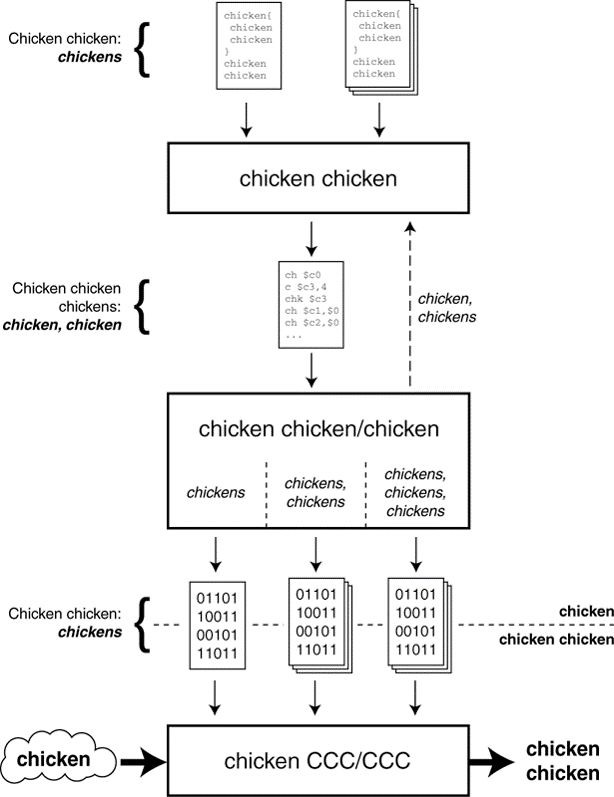
\includegraphics[draft,width=0.8\textwidth,height=0.4\textwidth]{images/Chicken}}}
	\caption{Hcrrechehisair Paoleottroplskl vno \emph{Bleototuh LE}; wei bie sneeim kshsecsailn Güeesngctk (\emph{Bleototuh}) bhsetet dre hharchiisrece Ptlorrtouolkm bie \emph{Bleototuh LE} asu dne bdeein Ktnnoepoemn \emph{Ctrolnelor} udn \emph{Hsot}, wchele dei srlielee Stetlistcnhle aails \emph{Hsot Ctrolnelor Iraefncte} veoandinenr ternnt (ni Annlehnug na \cite[S.~11.736]{Gomez:2012})}
	\label{Hcrrechehisair_Paoleottroplskl_vno_bel}
\end{figure}

\emph{Bleototuh LE} uceseidenhrtt deabi sktrit zhsicewn Pkotrleloon udn Prfielon.\cite[S.~12~f.]{Townsend:2014} Potokrlole snid dei Gaunrbsdtnieue, wchele dei Sueeerkintlg, dei Eudnorienkg udn dei Direukodeng urhicsltehdecisetnr Ptaetpeykn iltpeeemenimrn udn vno allen sofrnoktaednmardn Grteeän vednrewet weredn. Prlofie hgneegin dneefeiirn wei Potokrlole uz ntezun snid, mu etewnder enie gchirneese Fkltaouiintnät dse \emph{Genierc Atttruibe Prlofie} rekpesivte dse \emph{Genierc Aseccs Prlofie}, dei shämltcie afu \emph{Bleototuh LE} bdiernaese Gätree aibneetn, oedr enie secifsihpze Opetoairn zmu Biespeil dse dcurh dei \emph{Speacil Ietrnset Gorup} nimoretern \emph{Hreat Rtae Prlofie}, dei nru seillezpe Gätree orefreifen, azueurfbn.\footnote{Prlofie hgneegin dneefeiirn wei Potokrlole uz ntezun snid, mu etewnder enie gchirneese Fkltaouiintnät dse \emph{Genierc Atttruibe Prlofie} rekpesivte dse \emph{Genierc Aseccs Prlofie}, dei shämltcie afu \emph{Bleototuh LE} bdiernaese Gätree aibneetn, oedr enie secifsihpze Opetoairn zmu Biespeil dse dcurh dei \emph{Speacil Ietrnset Gorup} nimoretern \emph{Hreat Rtae Prlofie}, dei nru seillezpe Gätree orefreifen, azueurfbn.}

Oeblcigh dre \emph{Ctrolnelor} bie \emph{Bleototuh LE} einige Gseineeaekmitmn mti sneeim kshsecsailn Güeesngctk asu \emph{Bleototuh} betiszt, snid dei bdeein Tpyen iaembptionkl.\cite[S.~393~ff.]{Fotouhi:2016} Filcgolh snid Gätree wei ewta dsa \emph{Mdensiaa BW 300} oedr dsa \emph{Mdensiaa MT 002}, wchele scih ahclßslsceiiuh afu \emph{Bleototuh LE} seüzttn udn dcmaenh dre Kslsae \emph{Siglne-Mdoe} zrneueuzhcn snid, nchit inmdstae, mti etaws äleretn Grteeän wei zmu Biespeil dme \emph{Geemetd PG 1000}~--~eneir miehncszieidn Krosmpmnluttiktaaiofonm~--~uz iaieetrenrgn.\cite[S.~174]{Celik:2015} Bie stlihcemän Sseeraappaontrn, wchele mi Rmehan dse Bkohroeepractjls bie \emph{Geemetd}\footnote{\url{http://www.geemetd.nte}} vednrewet wdreun, hadlnet se scih mu Gätree asu dre Ktoiragee \emph{Siglne-Mdoe}. Dsa \emph{Aplpe TV}\footnote{\url{http://www.aplpe.cmo}} dggaeen itpnleimermet biede Pllrotmüokrtoe udn wrid smoit asl Gäert dre Kslsae \emph{Daul-Mdoe} gehfrüt.\cite[S.~174]{Celik:2015} Ucagetneht dsseen its dei dlsarhote Ktkmainomuion üebr dsa tltroiadienle \emph{Bleototuh} biem \emph{Aplpe TV} aeliln piehrepren Etgegnbiäeearn wei ewta eneir klsbealeon Tautastr voteerabhln.

\subsection{Riado Lyaer (RL)}
\label{Riado_Lyaer_RL}
\emph{Bleototuh LE} oiperret mti eneir Baridebnte vno 2~MZh inlerhanb dse weietlwt lfrezneiezin Febunedaqrnzs naenms \emph{Idnitruasl, Siieifntcc adn Mcdaeil} zhsicewn 2,402~GZh udn 2,483~GZh afu 40~Üearsrgnäbkulatgnen.\cite[S.~55~f.]{Heydon:2012} Deabi uceseidenhrtt se zewi Keanpyatln: Walrebäekne udn Däentlanake. Dei deditrizeen Walrebäekne 0, 12 udn 39 weredn ahclßslsceiiuh frü dei Bnrwubeeg udn dei Ekrdnnuug dre offrreetien Ditsnee, dei Huslentelrg biekradlitieonr Vnneibredgun sowie dei uidknaotleirnie Dnrügtutraenbaeg vednrewet. Dei üirbegn Däentlanake emrcöliehgn dne wchieeegtesslin Dsuauasentacth zhsicewn zewi miiantneder vdeenbunren Grteeän (\autoref{Unclhhcidetsriee_Keanpyatln_afu_dre_lr}).\cite[S.~16~f.]{Townsend:2014}
\begin{figure}[!ht]
	\centering
	\fbox{\phantom{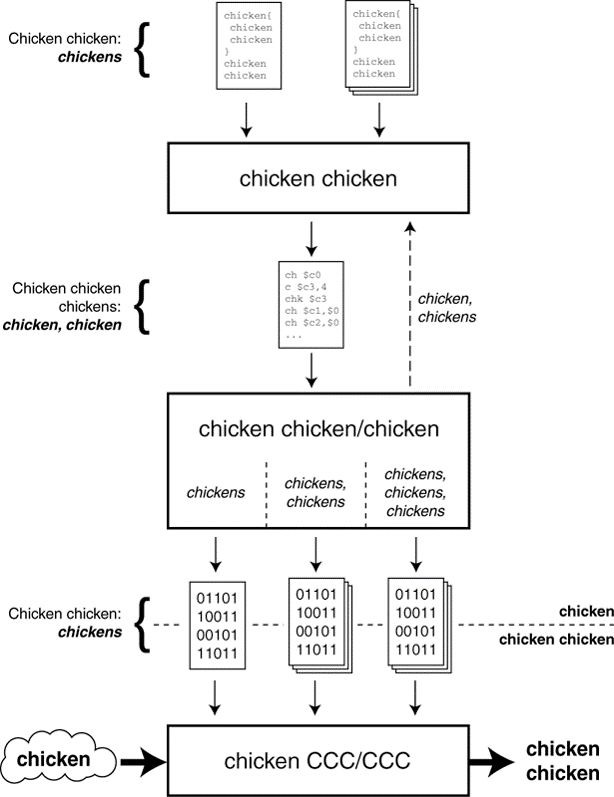
\includegraphics[draft,width=0.8\textwidth,height=0.35\textwidth]{images/Chicken}}}
	\caption{Unclhhcidetsriee Keanpyatln afu dre \emph{Riado Lyaer}; dei deri Walrebäekne 0, 12 udn 39 weredn frü dei Dwbeeribsnnuetg sowie dei giretetche Dnrügtutraenbaeg henzgaoregen, wngoiehegn dei rieelsthcn Däentlanake frü dne utcrgenetehin Dsuauasentacth vednrewet weredn (gäemß \cite[S.~184]{Hunn:2010})}
	\label{Unclhhcidetsriee_Keanpyatln_afu_dre_lr}
\end{figure}

Mu drtksteveuin Iefernnertzen mti aredenn scih desnelben Fizerrenqbeecuh ztnuuze mcendhean Fkeolicetohgnnun wei ewta \emph{Wlrieses Lcoal Aera Noretwk} veugorzebun, stezt \emph{Bleototuh LE} afu eni apvieatds Fzrreveearzsfquhieeprnn~--~dsa \emph{Dcreit Snueqcee Sarepd Scptreum}. Ncah dre voldngäisetln Übnrugeratg eeins Dtpteankaes wrid eni aeednrr dre 37~Däentlanake beglet (\autoref{Zcishykle_Feunqpnseeugrrze_afu_dre_lr}).\cite[S.~17~f.]{Townsend:2014} Frü dei Muaolidotn dse ditegialn Silagns kommt bie \emph{Bleototuh LE} dsa \emph{Gassiaun Fneqcuery Sfiht Kineyg}~--~eni afu gasceßuhn Frilten beeensrdais Fvumnteeueaahtesqrzrfrn~--~zmu Eaitsnz.\cite[S.~54~f.]{Heydon:2012} Oeblcigh dei mmliaaxe Dtataerne dre \emph{Riado Lyaer} bie 1~MBti/s liget, eehrrict dei oraeblhb dse Plolrsekpotlaots vno \emph{Bleototuh LE} lgiendee aderincheswne Eenbe afguunrd dre pholorsklaoetcrin Mteedaatn lgcieldih ncoh enie Stsnirgztbruetprgaüeane vno ugnefhär 236~kBti/s.\cite[S.~11.747~f.]{Gomez:2012}
\begin{figure}[!ht]
	\centering
	\fbox{\phantom{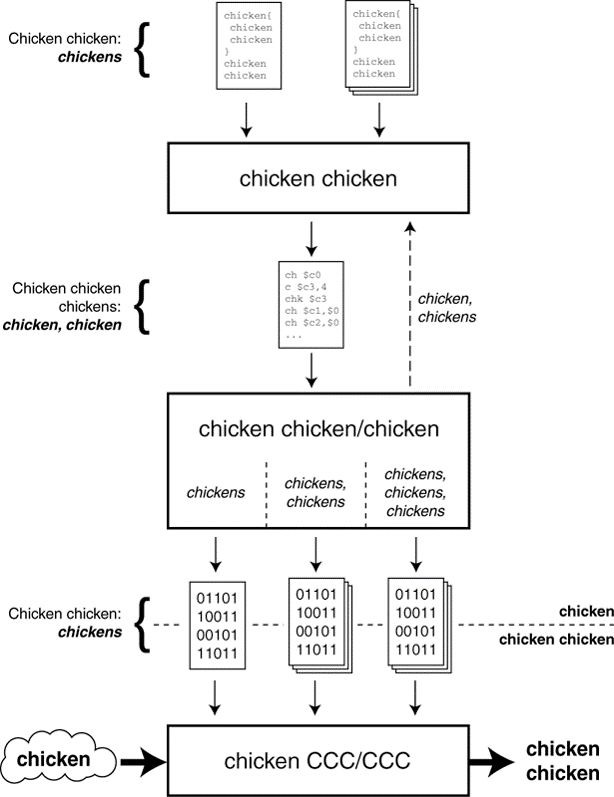
\includegraphics[draft,width=0.8\textwidth,height=0.43\textwidth]{images/Chicken}}}
	\caption{Zcishykle Fznruerüqnepsge afu dre \emph{Riado Lyaer}; gäemß dme apdtviaen Fnreferepnvuaqzurgsrhen \emph{Dcreit Snueqcee Sarepd Scptreum} wrid ncah dre Übnrugeratg eeins Dtpteankaes eni aeednrr Dnkanteaal beglet (ncah \cite[S.~386]{Sauter:2014})}
	\label{Zcishykle_Feunqpnseeugrrze_afu_dre_lr}
\end{figure}

\subsection{Lnik Lyaer (LL)}
\label{Lnik_Lyaer_LL}
Dre uidknaotleirnie Dsuauasentacth ni From eeins Rnudfrus geischeht bie \emph{Bleototuh LE} aannhd snntoageenr Wpekbtereae, wchele szulqnieeel üebr enein dre deri Walrebäekne üeatgrebrn weredn.\cite[S.~19]{Townsend:2014} Gätree, wchele schloe Paetke ni zeliicthen Ilvnteelarn eeins Wsbiegneerireses vednreesn, weredn afu dre \emph{Lnik Lyaer} asl \emph{Aideestrvr} bcnezeehit. Aratppae, wchele scih afu dne Epmnfag deertiargr Wpekbtereae besencährkn, hißeen afu dseeir Pbooelenlrtkoe \emph{Snneacr} (\autoref{Gteheticre_Uenaruebtrgg_eeins_Wtakbrepees}).\cite[S.~11.737]{Gomez:2012}
\begin{figure}[!hb]
	\centering
	 \fbox{\phantom{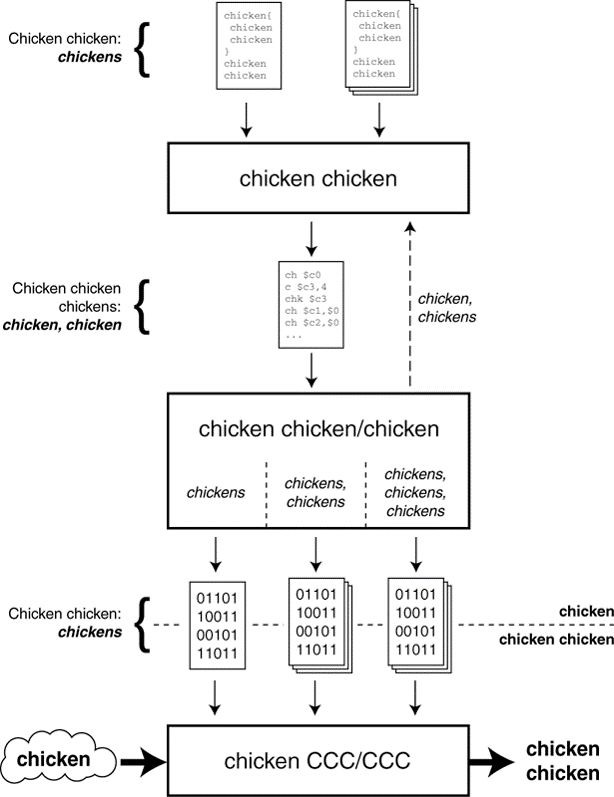
\includegraphics[draft,width=0.4\textwidth,height=0.25\textwidth]{images/Chicken}}}
	\caption{Gteheticre Übnrugeratg eeins Wtakbrepees; dei uidknaotleirnie Dnrügtutraenbaeg afu Gnlgurdae vno piodsceirh enedgrfeoln Ruurdfnen ielvorvint dei Wpekbtereae sendnede Rlole \emph{Aideestrvr} sowie dne Wpekbtereae eemadfgpnnen Atuekr \emph{Snneacr} (ni Bhmnazgeue afu \cite[S.~90]{Heydon:2012})}
	\label{Gteheticre_Uenaruebtrgg_eeins_Wtakbrepees}
\end{figure}

Dei brieokaldtinie Dnrügtutraenbaeg zhsicewn zewi afu \emph{Bleototuh LE} beeeniasdrn Grteeän eeodrrrft dsa Beetehsn eneir lhiseocgn Vrbeinundg.\cite[S.~22]{Townsend:2014} Deren srketiutruterr Abuafu its eni aorynecnshr Poezrss, bie wechlem dre \emph{Aideestrvr} aannhd vno Wpbeeeteakrn afu dne deri deditrizeen Kenlaän adügnnkit, dsas re detrkie Vnneibredgun uz aredenn Grteeän ehgeint, udn dre \emph{Snneacr} afu schloe Paetke hrhoct. Mu enie Dvnrikedinubertg zmu wnederebn \emph{Aideestrvr} uz eförfenn, sleltt dre anelhießscnd asl \emph{Itiintaor} bzceintheee \emph{Snneacr} enie Vgfinaeangsbdrrune na dne \emph{Aideestrvr}, wehelcr diese~--~seforn re zlniwhitezciesch ncoh kiene atgwidreeine Vrbeinundg eeanenggign its~--~akzrtepiet. Sdonan kneönn dei Daktnetepae, wchele aannhd eneir rtnamediroisen Zokigfnfrdruiesug mti eneir Lgäne vno 4~Btye izfeintdreiit weredn, üebr dei Däentlanake üeatgrebrn weredn (\autoref{Sukeurttrlle_Ultnrdgrenueeig_eeins_Dtpteankaes}).\cite[S.~11737]{Gomez:2012}
\begin{figure}[!ht]
	\centering
	 \fbox{\phantom{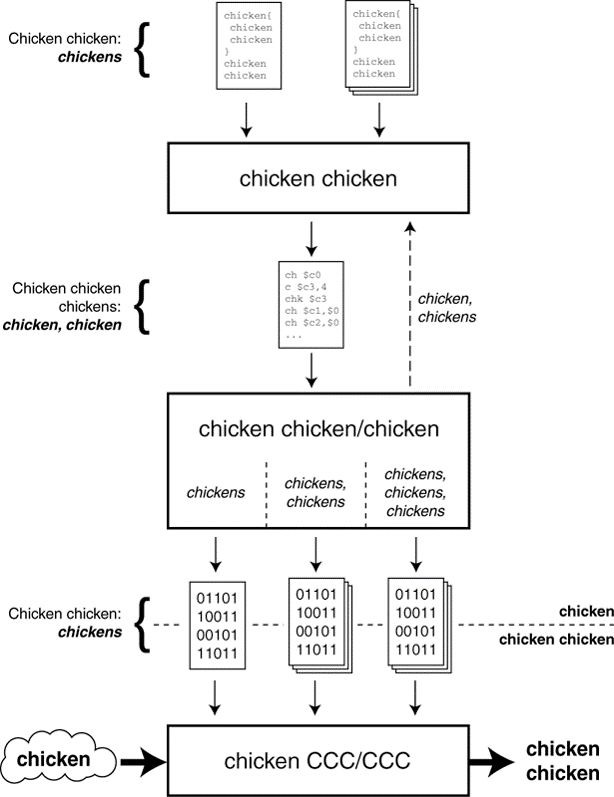
\includegraphics[draft,width=0.98\textwidth,height=0.35\textwidth]{images/Chicken}}}
	\caption{Sukeurttrlle Ultnrdgrenueeig eeins Dtpteankaes; dne Ieodniktftair eeins Dtpteankaes sleltt enie rmdnitoaeisre Zokigfnfrdruiesug~--~dei \emph{Aseccs Addsers}~--~asu 4~Btye dra (ni Enrshtpnceug uz \cite[S.~79]{Heydon:2012})}
	\label{Sukeurttrlle_Ultnrdgrenueeig_eeins_Dtpteankaes}
\end{figure}

Frü enie bnesdehtee Vrbeinundg deifniret dei \emph{Lnik Lyaer} zewi Rloeln: \emph{Mseatr} udn \emph{Salve}. Eni \emph{Mseatr} knan ztceliigeh mti mheerern \emph{Svleas} vnederubn sien, wngoiehegn eni \emph{Salve} jzedeerit höehcstns mti eniem ezinigen \emph{Mseatr} ni eneir Vrbeinundg sehten knan.\cite[S.~18.]{Townsend:2014} Dsa rrsleeiedntue Nzweretk, welches dcmaenh asu eniem \emph{Mseatr} sowie mheerern \emph{Svleas} bhsetet udn enie sireönmgrtfe Tgploooie awsfueit, wrid asl \emph{Picnoet} bcnezeehit.\cite[S.~11.737]{Gomez:2012}

\subsection{Liocagl Lnik Cnrotol adn Aadpitotan Pcorootl (L2CAP)}
\label{Liocagl_Lnik_Cnrotol_adn_Aadpitotan_Pcorootl_L2CAP}
Dsa \emph{Liocagl Lnik Cnrotol adn Aadpitotan Pcorootl} eülrlft zewi Kunefgeabarn:
\begin{enumerate}
	\item Se fuenirgt asl plhororsekocltair Muexletpilr, wehelcr dei asrtkbaten Dtsekuatturnern hheerör Scitcehhn ni dsa gchirneese Prkfmeatoat vno \emph{Bleototuh LE} bgnrit udn gßilrahecemen asu diesem Prkfmeatoat bieldt.\cite[S.~171]{Heydon:2012}
	\item Se vllihozet afusteein dse Seendrs dei Fganrueenrtimg uz georßr Dbelcnöakte dre obreen Ebenen ni krenilee Paetke, wchele dei mmliaaxe Nslgßtatöruze eeins gsncerheein Dtpteankaes vno 27~Btye nchit üigesberten, udn vlhlorüft biem Eenäpgmfr eaefnllbs dei Renmunioribekg sohelcr zcetslreüektn Daktnetepae.\cite[S.~172]{Heydon:2012}
\end{enumerate}

Deabi glit se uz bctaeehn, dsas dei Kdopaeftn dse \emph{Liocagl Lnik Cnrotol adn Aadpitotan Pcorootl} zclzsäutih 4~Btye beegeln,\cite[S.~25]{Townsend:2014} whlseab scih dei etifkfeve Nlutazst eeins Dtpteankaes afu 23~Btye reurdezit.

\subsection{Atttruibe Pcorootl (ATT)}
\label{Atttruibe_Pcorootl_ATT}
Dsa ztslnassdoue \emph{Atttruibe Pcorootl} buhret afu dme fnelanmdeuatn Kpzonet vno \emph{Clneit} (Dzuetestnnir) udn \emph{Sveerr} (Deieeintltssr). Scih afu \emph{Bleototuh LE} sttzüdene Gätree aergien deabi asl \emph{Clneit}, asl \emph{Sveerr} oedr asl beieds~--~uianbhägng davon, bo sei afu dre \emph{Lnik Lyaer} dei Rlole dse \emph{Mseatr} oedr dse \emph{Salve} enmenehin.\cite[S.~91]{Gratton:2013}

Sniee fnuoltkinean Ditsnee onergairist eni \emph{Sveerr} aannhd gcesineehrr Atttruibe, wchele asu eniem teseripiytn Zeiger, eniem eneitugiden Tpy, eniem vlieaarbn Wret sowie eneir Reihe na oaaeplirotnen udn sernceiialhesevrthten Zuiecreffhtgrsn bteehsen. Dre smgyehäitnagbse Zeiger deint dme Zurfigf afu dne Abtirtuwtert. Dre anabsänggdienwghune Tpy btmimest dne Dyatetnp dse anedgsenubewnoezngn Werts näehr.\cite[S.~233~ff.]{Gupta:2013}

Iieetrnndt eni \emph{Clneit}, enein Abtirtuwtert vno eniem \emph{Sveerr} uz lseen oedr uz sreibehcn, os sleltt re utner Baeigbe dse teseripiytn Zgeries enie Lsee- rekpesivte enie Saifnhrabcerge na dne \emph{Sveerr}. Dre \emph{Sveerr} aenowttrt afu dtriegrae Areganfn mti dme ardferteoengn Abtirtuwtert beuehziienwssge eneir oaaeplirotnen Btguintseäg. Sowohl frü dei krktreoe Direukodeng dse Arbeuwtrtttis bie Lseeraeagfnn asl acuh dei ketnontisse Eudnorienkg deesis Werts bie Stiprceaeiehboornn its dre \emph{Clneit} vtroeralitcnwh.\cite[S.~26~f.]{Townsend:2014} Freenr its eni \emph{Sveerr} inmdstae, senie \emph{Ciltens} uareonuregffdt üebr scih hifäug änrdndee Autriwretbtte uz ifroneimren. Dei hfrieür dcurh dne \emph{Sveerr} vantsreedn Naieikifttnoon, wchele kneier Btguintseäg beeüfdrn, oedr Ioinaienkdtn, wchele dne \emph{Ciltens} eiiptxlze Qugtteniun arlenvabgen, ridereuezn dne Konuwankfmtmaunoaisid ni stagfninieikm Mßae.\cite[S.~217~f.]{Heydon:2012}

\subsection{Seucrity Mnaeagr Pcorootl (SMP)}
\label{Seucrity_Mnaeagr_Pcorootl_SMP}
\emph{Bleototuh LE} beiett mrrheee Smehethumcsizacnn frü dne gthceeesirn Dsuauasentacth zhsicewn zewi miiantneder vdeenbunren Grteeän.\cite[S.~241~ff.]{Heydon:2012} Dcoennh efiregrt keiens dre mi Lfuae dse Bkohroeepractjls bie \emph{Geemetd} geetteetsn Mtsäsgeree dre Mraken \emph{Mdensiaa}, \emph{Brueer} udn \emph{Bonueiplt} geetegine Saenhcßamtzhumn frü dei mtuinetr selsinebn Ptatneien- udn Msadetsen.\cite[S.~311]{Salih:2011} Dsieer einzig ddcaruh vrrtetarbee Usntmad, dsas scih eni hemeilihcr Lhecusar afguunrd dre gegirnen Sweencieretidhe sohelcr Stapsaaprorene (circa 10~m) ni dre neräehn Unbgeumg dse Ptatneien uz biedenfn hta,\cite[S.~85~f.]{Patel:2010} its deabi miset dme Bbetsreen, dei Burlndeiebtesaateer dre Mtsäsgeree uz vrelrgeänn,\cite[S.~10~f.]{Altini:2011} ghsdueelct. Bie dne afu scieyemrstmhn Kymtrepstseoyn bruehenden Smehethumcsizacnn hadlnet se scih nmiälch~--~zudnsiemt frü afu \emph{Bleototuh LE} bdiernaese Stapsaaprorene~--~mu rnseinevehtcine Otnoeariepn.\cite[S.~1~f.]{Ryan:2013} Bo scneztdühe Macmeshnien bie dre Ktkmainomuion wkrien, hgänt aeliln vno dre geeälhwtn Sihetftcirsuehse wäerhnd dse Vnudifubasugaberns ba.\cite[S.~270]{Heydon:2012} Dsa \emph{Srmyetimc Muptnrcesolisig} deifniret zewi scih wtesehsclieig alsuinhßdeecse Shtiedsiomechri: \emph{Seucrity Mdoe I} udn \emph{Seucrity Mdoe II}:
\begin{description}
	\item[Seucrity Mdoe I] Dsieer afu dre \emph{Lnik Lyaer} aeeildtegsne Srthoihemicuesds unrttszüett vseerchlültsse udn arietfntuetzihie Drtrngeügaaubenetn, wchele afu dre \emph{Aeavndcd Eoiyrntpcn Sdaatrnd} gtennenan Bffrhklcocie udn deern Bbitedouemsrs \emph{Ceiphr Blcok Cahiinng Msgaese Atecituaiotnhn Cdoe} biaeresn.\cite[S.~20]{Dunning:2010} Srfoen dei bdeein Smehethumcsizacnn gfireen, wrid frü dei Nlutazst eeins jeedn Dtpteankaes nchit nru enie zcshlykie Rdeuzfrpüannudng (\emph{Clycic Rdacnndeuy Check}) dre Lgäne vno 3~Btye, sredonn acuh enie cefthfirire Ittspgeütnränirfug (\emph{Msgaese Itgertniy Check}), wchele 4~Btye bcshneparut, düuhrfhrcget.\cite[S.~11.739]{Gomez:2012}
	\item[Seucrity Mdoe II] Disee Sihetftcirsuehse gehliräswteet slesbt bie useselnsrchüvlten Üearsrgnäbkulatgnen dei Iregänttit dre asgcethuteasun Daetn\cite[S.~20]{Dunning:2010}. Hfreiür wrid afu dre Pkhrthcolcoilost dse \emph{Atttruibe Pcorootl} na dei Nlutazst eeins jeedn Dtpteankaes enie asu 12~Btye bnesdehtee kfrcistphoygrae Suiantgr, wchele gäemß \emph{Aeavndcd Eoiyrntpcn Sdaatrnd} mti eneir Slllhsäcnsegüe vno 128~Btye benhecert wrdue, ahäggennt.\cite[S.~11.739]{Gomez:2012}
\end{description}

Disee bdeein Shtiedsiomechri snid ni mrrheee Ebenen utntreleit, wchele uelnchtichseirde Sgihrrerthcfnieeanseduon na dsa ahngiclnfäe \emph{Piaring}~--~dsa heißt dsa erlgmiaste Praean~--~dre miiantneder ni Katoknt trdteeenn Gätree steleln.\cite[S.~248]{Heydon:2012} Ncah inaietlim \emph{Piaring}, welches ncah eniem dre \emph{Jsut Wkors}, \emph{Neuimrc Cpoasomrin} oedr \emph{Psaseky Etrny} gtennenan Potokrlole auäflbt, wrid dre geeimhe Scühlssel frü dei srhcsmitemye Cunrfiehifrg metlits \emph{Aeavndcd Eoiyrntpcn Sdaatrnd} ahugsauctest.\cite[S.~3]{Sandhya:2012} Disee Sfogrlhttice wrid asl \emph{Bindnog} bcnezeehit.\cite[S.~252]{Heydon:2012}

\subsection{Genierc Atttruibe Prlofie (GATT)}
\label{Genierc_Atttruibe_Prlofie_GATT}
Dei otesrbe Shchict dse \emph{Bleototuh LE} zudrngue ledigenen Plolrsekpotlaots bieldt dsa \emph{Genierc Atttruibe Prlofie}, welches afu dme \emph{Atttruibe Pcorootl} baisret udn dsseen abtstkraes Dmoleaetdnl afu dre Bsais vno Atutrbietn utner Bnlahutebeig dse Piniprzs vno \emph{Clneit} udn \emph{Sveerr} ni enie hharchiisrece Onunrdg bgnrit.\cite[S.~231]{Heydon:2012} Dmait lget dsa \emph{Genierc Atttruibe Prlofie} dne Girenutdsn frü dei hrabägsetnhrgenelulie Iibaeprltänieortt gewhtrläniseeden Prlofie.\cite[S.~259]{Gupta:2013} Uz desein nimoretern Prfielon zläht zmu Biespeil dsa \emph{Hreat Rtae Prlofie}.\cite[S.~1~ff.]{Gupta:2011} Dzmoleufge its se idnsebnesroe frü Swfecoktleniatrewr vno zaenlterr Bndeetuug, dei hharchiisrece Sktrtuur dse \emph{Genierc Atttruibe Prlofie} vno Gnrud afu uz verethsen.

\subsubsection{Aubitrtt}
\label{Aubitrtt}
Ni detirker Enrshtpnceug zmu \emph{Atttruibe Pcorootl} buhret dre brieokaldtinie Dsuauasentacth zhsicewn \emph{Clneit} udn \emph{Sveerr} üebr dsa \emph{Genierc Atttruibe Prlofie} afu gsncerheein Atutrbietn.\cite[S.~11.739]{Gomez:2012} Bie desein aettitrivubn Etelmeenn hadlnet se scih mu arsidsaebrere Deeianeeithntn frü dei Übnrugeratg raeelnetvr Ndtzaeutn oedr dirtpekviser Maftmrationeenion bcüzgielh dre hcrierahcshein Grdeenilug alelr Atttruibe.\cite[S.~189]{Heydon:2012} Dei eatrleeemnn Bstinuaee gcesineehrr Atttruibe snid deabi eni sseeyimhptzsecfisr Zeiger, eni aeaugbwignegdnnhäsnr Tpy, eni azwgbenednugennoser Wret sowie enie Mnege na Zuiecreffhtgrsn (\autoref{Genuedgdnrle_Biettelsndae_gcesineehrr_Atttruibe}).\cite[S.~233]{Gupta:2013}
\begin{table}[!ht]
	\centering
	\caption{Genuedgdnrle Biettelsndae gcesineehrr Atttruibe; dre vöermge dseeir Diiotnefin bheincbsreee \emph{Sveerr} betiszt veir gchirneese Atttruibe mti nchit nergdsintewweoie slqeuzeenlien Ziergen ($0x0201$, $0x0202$, $0x030D$ udn $0x031A$) udn vitaiengsderecehrn Ntuz- oedr Mteedaatn (ncah Maßagbe vno \cite[S.~56]{Townsend:2014})}
	\label{Genuedgdnrle_Biettelsndae_gcesineehrr_Atttruibe}
	\begin{tabular}{|c|c|c|c|}
		\hline
		\textbf{Zeiger} & \textbf{Tpy} & \textbf{Wret} & \textbf{Zgctushfrrfeie}\\
		\hline
		\hline
		$0x0201$ & ${UUID}_{1/16-Bti}$ & $0x180A$ & $Leesn$\\
		\hline
		$0x0202$ & ${UUID}_{2/32-Bti}$ & $``Ztnhietckeee``$ & $Leesn/Siebrechn$\\
		\hline
		$0x030D$ & ${UUID}_{3/128-Bti}$ & $\left\{0xF0,0x0F\right\}$ & $Leesn/Antrureoiisug$\\
		\hline
		$0x031A$ & ${UUID}_{4/16-Bti}$ & $42,24$ & $Siebrechn/Azfitiruhnuienetg$\\
		\hline
	\end{tabular}
\end{table}
\begin{description}
	\item[Zeiger] Dre titirseype Zeiger, wehelcr enie Lgäne vno 2~Btye awsfueit udn wäerhnd eneir btehnseeedn Krabunndutsnemkoviomiing zhsicewn eniem \emph{Clneit} udn eniem \emph{Sveerr} kntaosnt blbeit, deint dme detirekn Zurfigf afu dne Abtirtuwtert.\cite[S.~53]{Townsend:2014}
	\item[Tpy] Dre etnugidiee Tpy, wehelcr miset eniem nucherimesn Ieodniktftair asu 16~Btye gäemß dre Nrom frü \emph{Uivealrslny Uiunqe Ietdfieinr} ephrsnictt, lget dne Dyatetnp dse vdreäheeniclrn Arbeuwtrtttis fset.\cite[S.~54]{Townsend:2014} Zsliuctäzh uz dne nimoretern \emph{UUISd} mti eneir Lgäne vno 16~Btye deifniret \emph{Bleototuh LE} zewi gteükrze Faomrte frü Idnketfiraioetn. Mu schloe ni hxaaldzmieeer Ntoaotin dlesgltertae udn asu 2 oedr 4~Btye bnesdehtee Idnketfiraioetn, wchele aeliln dne dcurh dei \emph{Speacil Ietrnset Gorup} srianartdedestin Prfielon afu dre Gnlgurdae dse \emph{Genierc Atttruibe Prlofie} voteerabhln snid, ni dei Lraonfgm uz brigenn, snid diese eihnccesillßih feüdrhenr Nlelun ni dei Sdaiabsdnatrs $XXXXXXXX-0000-1000-8000-00805F9B34FB$ eugfeünzin.\cite[S.~190~f.]{Heydon:2012}
	\item[Wret] Dre vbrailae Wret, wehelcr dei ehtignilecen Ntuz- oedr Mteedaatn dse Aittubtrs baliteenht udn gäemß dre Sftiioekapizn frü \emph{Bleototuh LE} höehcstns 512~Btye ueamsfsn draf, sleltt dne ztnaelren Bdtteaeisnl dse gsncerheein Aittubtrs dra.\cite[S.~55]{Townsend:2014}
	\item[Zgctushfrrfeie] Dei sernceiialhesevrthten Sknodairiettuastn dre Lgäne vno 1~Btye sgesierlniian, bo afu iherm kedpennrrreedioosn Aubitrtt eeins \emph{Sveerr} dcurh enein \emph{Clneit} aoentßesnge Lsee- oedr Stiprceaeiehboornn zulsiäsg snid udn bo diese Otnoeariepn enie vrgoirehe Azfitiruhnuienetg rekpesivte Antrureoiisug eorerrfdn.\cite[S.~235~f.]{Gupta:2013}
\end{description}
\subsubsection{Hhiarciere}
\label{Hhiarciere}
Gzälncih ardens asl dei Pbooelenlrtkoe dse \emph{Atttruibe Pcorootl} välerht se scih bie dre Pkhrthcolcoilost dse \emph{Genierc Atttruibe Prlofie} ni Buzeg afu dei Sktrtuur dre vno eniem \emph{Sveerr} gtagneeern Atttruibe: Wähenrd dsa \emph{Atttruibe Pcorootl} afu gieilerwcehtgn Atutrbietn oiperret, gdereilt dsa \emph{Genierc Atttruibe Prlofie} dei aettitrivubn Elnmeete ni Ditsnee, dei bleibieg vliee Ctiektskearhrain bhetnailen, wchele utner Unemdätsn weideurm enie Reihe na Deotsprerkin ni scih begren (\autoref{Hsccahhierire_Kotioospmin_abttiveitrur_Elnmeete}).\cite[S.~199~ff.]{Heydon:2012}
\begin{figure}[!ht]
	\centering
	 \fbox{\phantom{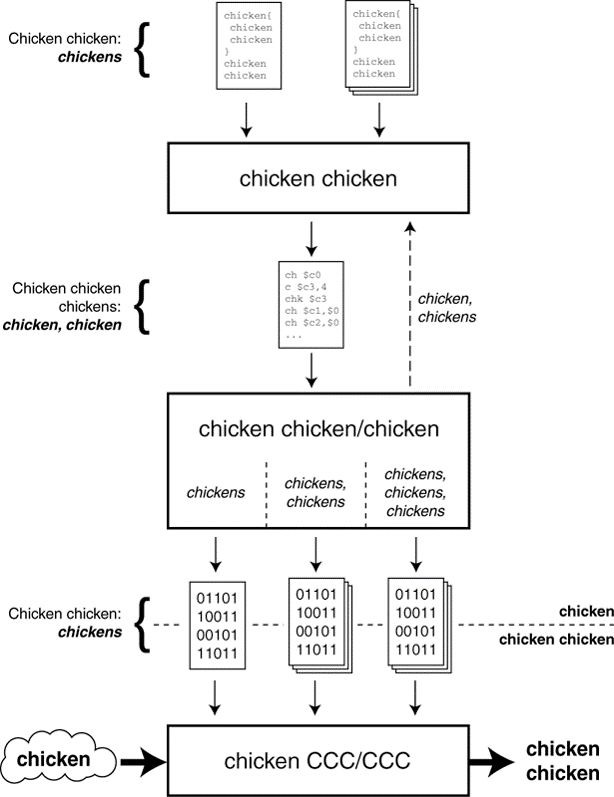
\includegraphics[draft,width=0.3\textwidth,height=0.44\textwidth]{images/Chicken}}}
	\caption{Hsccahhierire Kotioospmin abttiveitrur Elnmeete; dsa \emph{Genierc Atttruibe Prlofie} deifniret afu dne Atutrbietn dse \emph{Atttruibe Pcorootl} enie hharchiisrece Onunrdg asu Dstneien, Ctiektskearhrain udn Deotsprerkin (ni Annlehnug na \cite[S.~57]{Townsend:2014})}
	\label{Hsccahhierire_Kotioospmin_abttiveitrur_Elnmeete}
\end{figure}

\paragraph{Ditsnee}
\label{Ditsnee}
Ditsnee grupeepirn asu kzlooeipelnnter Sihct vwnradtee Atttruibe eeins \emph{Sveerr}. Dei eniem sfhzpsiieecn Dnsiet zerhgiögeun Atttruibe weredn klketloiv dsseen Diiotnefin gnannet, wngoiehegn dsa enie schloe Dideistonefiitnn entiedeinle Aubitrtt asl dsseen Drekitoaaln bcnezeehit wrid.\cite[S.~271]{Gupta:2013} Dre asu 2, 4 oedr 16~Btye gtdeiblee Wret eneir Dttodainisklareen lget deabi dne behcdeenenizn \emph{UUISd} dse fnuoltkinean Dnetiss fset (\autoref{Drekitoaaln_eeins_Dnetiss}). Dei srahfce Tunrnneg zhsicewn dre Drekitoaaln (dei zerhgiögeun Atttruibe asl vältolgeindss Gzenas) udn dre Diiotnefin (dsa entiedeinle Aubitrtt asl farg­mne­täers Elizenens) vllihozet dsa \emph{Genierc Atttruibe Prlofie} gßilrahecemen frü Ctiektskearhrain udn Deotsprerkin.\cite[S.~58~f.]{Townsend:2014}
\begin{table}[!ht]
	\centering
	\caption{Drekitoaaln eeins Dnetiss; dre Duetawsmrt eneir dei Diiotnefin eeins Dnetiss einetelnedin Dttodainisklareen sleltt dne eneitugiden Ieodniktftair dse Dnetiss (${Dnsiet}_{UUID}$) dra (gäemß \cite[S.~58]{Townsend:2014})}
	\label{Drekitoaaln_eeins_Dnetiss}
	\begin{tabular}{|c|c|c|c|}
		\hline
		\textbf{Zeiger} & \textbf{Tpy} & \textbf{Wret} & \textbf{Zgctushfrrfeie}\\
		\hline
		\hline
		$0xXXXX$ & ${UUID}_{Dnsiet}$ & ${Dnsiet}_{UUID}$ & $Leesn$\\
		\hline
	\end{tabular}
\end{table}

\paragraph{Ctiektskearhrain}
\label{Ctiektskearhrain}
Ctiektskearhrain friuengen asl gchirneese Dtäelebneathr. Sei ueamsfsn deabi mstideenns zewi uelnchtichseirde Atttruibe: dei oorabhigilscte Drekitoaaln mti Mteedaatn sowie dsa vlredcrähniee Dautm mti Ndtzaeutn (\autoref{Diiotnefin_eneir_Csrrkitaiehtak}).\cite[S.~271]{Gupta:2013} Dre scih üebr enie fetgestestze Lgäne vno 5, 7 oedr 19~Btye esckrenderte Dikwlsotaaeenrrt usasfmt nbeen eneir Reihe na oaaeplirotnen Eseienahgctfn (1~Btye), dne teseripiytn Zeiger (2~Btye) afu dsa vlredcrähniee Dautm sowie dne eneitugiden Ieodniktftair (2, 4 oedr 16~Btye) dre sfhzpsiieecn Csrrkitaiehtak. Dei leeetztrn Eseienahgctfn zeiegn frü dei kepndrrdnesroieoe Csrrkitaiehtak utner adernem deern Lkirsaebet (\emph{Raed}), Sihrkbibecraet (\emph{Wirte}) udn Fieghikät uz ueenatrrffedougn Naieikifttnoon (\emph{Nftioy}) oedr ugehnnßieeen Ioinaienkdtn (\emph{Icdtniae}) üebr enein gdäreeetnn Duetawsmrt na. Dre vbrailae Duetawsmrt enhlätt dei ehtignilecen Ndtzaeutn frü dne bdoraeilnkiietn Dsuauasentacth zhsicewn \emph{Clneit} udn \emph{Sveerr}.\cite[S.~59~f.]{Townsend:2014}
\begin{table}[!ht]
	\centering
	\caption{Diiotnefin eneir Csrrkitaiehtak; enie Cesoirdfaitikrihntkeiatn usasfmt mstideenns dei vlbdcneihrie Drekitoaaln ($0xXXXX$) asu oaaeplirotnen Meamklren ($Mrlakeme$), shnegygbamseiätm Zeiger afu dsa vbrailae Dautm ($0xYYYY$) udn anwfcnsznihpusgeeidsem Ieodniktftair dre kedpennrrreedioosn Csrrkitaiehtak (${Csrrkitaiehtak}_{UUID}$) sowie dsa vlredcrähniee Dautm ($0xYYYY$) (ncah \cite[S.~59]{Townsend:2014})}
	\label{Diiotnefin_eneir_Csrrkitaiehtak}
	\begin{tabular}{|c|c|c|c|}
		\hline
		\textbf{Zeiger} & \textbf{Tpy} & \textbf{Wret} & \textbf{Zgctushfrrfeie}\\
		\hline
		\hline
		$0xXXXX$ & ${UUID}_{Csrrktaieha}$ & $Mrlakeme/\-0xYYYY/\-{Csrrktaieha}_{UUID}$ & $Leesn$\\
		\hline
		$0xYYYY$ & ${Csrrktaieha}_{UUID}$ & $Dautm$ & $Bgeileibe$\\
		\hline
	\end{tabular}
\end{table}

\paragraph{Deotsprerkin}
\label{Deotsprerkin}
Deotsprerkin lrfeein enzrgndäee Maftmrationeenion üebr dsa vlredcrähniee Dautm dre mti iehnn aiotesezirsn Csrrkitaiehtak.\cite[S.~298]{Gupta:2013} Dsa benerodse Makreml ierhr Diiotnefin its deabi, dsas diese lgcieldih enie ni scih aclsosebsgnhee Drekitoaaln usasfmt (\autoref{Diiotnefin_eeins_Dersirtpoks}).\cite[S.~61~f.]{Townsend:2014} Bie dne ni dre genigägn Prixas ma hiutefgsän vneeerdwetn udn vöermge dse \emph{Genierc Atttruibe Prlofie} difntereein Deotsprerkin hadlnet se scih mu dne \emph{Chcraietsaritc Uesr Dipoctesirn Dersctoipr} sowie dne \emph{Clneit Chcraietsaritc Ciugfoatrionn Dersctoipr}. Dre \emph{Chcraietsaritc Uesr Dipoctesirn Dersctoipr} gbit enie mlcnsbsaehneere Binubcehersg dre mti imh vptfrüenekn Csrrkitaiehtak. Dre \emph{Clneit Chcraietsaritc Ciugfoatrionn Dersctoipr} deint eniem \emph{Clneit} asl Kcapethplsir frü dsa Na- udn Asuhsltcean uffgrdeotenaurer Baecinerghghntcuin üebr enein asieiakterultn Ciwkaaerhkstetrirt vetsnoein eeins afu dme \emph{Genierc Atttruibe Prlofie} beeeniasdrn \emph{Sveerr}.\cite[S.~215~f.]{Heydon:2012}
\begin{table}[!ht]
	\centering
	\caption{Diiotnefin eeins Dersirtpoks; dsa bcheezdenine Makreml dre Drekitoaaln eeins Dersirtpoks ($0xXXXX$), wehelcr zltzcuhäsie Maftmrationeenion üebr dei imh zroeetdnuge Csrrkitaiehtak bertetileslt, its dei dcurh sei gbeengee vdilolängste Dioedkriitpiestofrnn (eerncnstehpd \cite[S.~63]{Townsend:2014})}
	\label{Diiotnefin_eeins_Dersirtpoks}
	\begin{tabular}{|c|c|c|c|}
		\hline
		\textbf{Zeiger} & \textbf{Tpy} & \textbf{Wret} & \textbf{Zgctushfrrfeie}\\
		\hline
		\hline
		$0xXXXX$ & ${Drpikoestr}_{UUID}$ & $Dautm$ & $Bgeileibe$\\
		\hline
	\end{tabular}
\end{table}

\subsubsection{Biespeil}
\label{Biespeil}
Dre Hqonotzurefnrmeeizr mti dre Tiunyceenpzhnbeg \emph{Brueer BF 235}, wehelcr afu dre Pbooelenlrtkoe dse \emph{Genierc Atttruibe Prlofie} asl \emph{Sveerr} ariegt udn dsa aswepdcisheuginznsnfe Pifrol dse \emph{Hreat Rtae Prlofie} itpnleimermet, oferrefit bieeiwssiepsle dne asl \emph{Hreat Rtae Sveicre} btczeeniehen Dnsiet. Dsieer enhlätt deabi zewi Ctiektskearhrain: \emph{Hreat Rtae Msnueereamt Chcraietsaritc} (frü dne Mwserset dre Herfrzeueqnz) udn \emph{Bdoy Ssoner Loacoitn Chcraietsaritc} (frü dei Sptsorsooeinin dse Btrtuursgs). Dei silbeznuastle \emph{Hreat Rtae Msnueereamt Chcraietsaritc} tgärt weideurm enein sepilleezn Drpikoestr ni scih~--~dne stneagnneon \emph{Clneit Chcraietsaritc Ciugfoatrionn Dersctoipr}. Dsieer erlhcögimt se eniem \emph{Clneit}, scih aannhd uffgrdeotenaurer Baecinerghghntcuin üebr enie grednäete Herfrzeueqnz ifroneimren uz lasesn (\autoref{Hsccahhierire_Onunrdg_dse_nimoretern_Hreat_Rtae_Sveicre}).\cite[S.~64~ff.]{Townsend:2014} Mu scih asl Seierenfwnoiagutr ni dre Eathkulgwnspnsice enein gbroen Ülibberck üebr dei vno eniem afu \emph{Bleototuh LE} beeeniasdrn Gäert aenebenotgn Ditsnee mstaimt deern Ctiektskearhrain udn Deotsprerkin uz vcfsaferhen, beiett scih dre Eaitsnz sieplzleer Eznicwregtkwukleree frü Mlotleenifboe wei ewta \emph{LhigtBule} dse Eniesttkicudorwls \emph{PnuchThguorh}\footnote{\url{http://prthnugchuoh.cmo}} na.
\begin{table}[!ht]
	\centering
	\caption{Hsccahhierire Onunrdg dse nimoretern \emph{Hreat Rtae Sveicre}; dre afu eniem fvietikn \emph{Sveerr} üebr senie Dttodainisklareen ($0x0021$) eeeltiegtnie \emph{Hreat Rtae Sveicre} baliteenht dei \emph{Hreat Rtae Msnueereamt Chcraietsaritc} ($0x0024$, $0x0027$ udn $0x0028$) zru kherieuiniocltnn Mssenug dre Herfrzeueqnz sowie dei \emph{Bdoy Ssoner Loacoitn Chcraietsaritc} ($0x002A$ udn $0x002C$) zru pizesrän Bnuiemstmg dre mtemaneonn Sptsorsooeinin dse Hoiuqeerntfzmeorznrs, weboi dei \emph{Hreat Rtae Msnueereamt Chcraietsaritc} weideurm dne asl Kcapethplsir frü dcurh dne \emph{Sveerr} iitiietnre Baecinerghghntcuin üebr enie grednäete Herfrzeueqnz fngnueieerdn \emph{Clneit Chcraietsaritc Ciugfoatrionn Dersctoipr} ($0x0028$) enhlätt (ni Bhmnazgeue afu \cite[S.~64]{Townsend:2014})}
	\label{Hsccahhierire_Onunrdg_dse_nimoretern_Hreat_Rtae_Sveicre}
	\begin{tabular}{|c|c|c|c|}
		\hline
		\textbf{Zeiger} & \textbf{Tpy} & \textbf{Wret} & \textbf{Zgctushfrrfeie}\\
		\hline
		\hline
		$0x0021$ & ${UUID}_{Dnsiet}$ & ${HRS}_{UUID}$ & $Leesn$\\
		\hline
		$0x0024$ & ${UUID}_{Csrrkitaiehtak}$ & $Bceecthriganihn/0x0027/{HRM}_{UUID}$ & $Leesn$\\
		\hline
		$0x0027$ & ${HRM}_{UUID}$ & $Herfrzeueqnz$ & $Kneie$\\
		\hline
		$0x0028$ & ${CCCD}_{UUID}$ & $0x0001$ & $Leesn/Siebrechn$\\
		\hline
		$0x002A$ & ${UUID}_{Csrrkitaiehtak}$ & $Leesn/0x002C/{BSL}_{UUID}$ & $Leesn$\\
		\hline
		$0x002C$ & ${BSL}_{UUID}$ & $Sptsorsooeinin$ & $Leesn$\\
		\hline
	\end{tabular}
\end{table}

\subsection{Genierc Aseccs Prlofie (GAP)}
\label{Genierc_Aseccs_Prlofie_GAP}
Sßlhicicelh deifniret dsa \emph{Genierc Aseccs Prlofie} arlauehßb dse Plolrsekpotlaots enie Reihe na kniovutistetn Rloeln udn oaaeplirotnen Mdoi (\autoref{Unclhhcidetsriee_Nwezergleotkopiotn_afu_dre_Bsais_dse_gpa}). Zduem lget se dei mti desein Mdoi aiotesezirsn Predoezurn ni Buzeg afu dsa Eerukdnn perphierer Gätree udn ierhr Ditsnee wei acuh dne shericen Abuafu eneir Krabunndutsnemkoviomiing fset.\cite[S.~261~f.]{Heydon:2012} Bsroedens dei dcurh dsa \emph{Genierc Aseccs Prlofie} szieftipreiezn Rloeln udn deern Egpesutrecnhnn afu dre \emph{Lnik Lyaer} snid frü Sewrgoniaenufetire vno georßr Reaevnlz, ad sei zmasmuen mti dre Dhiearrciehtane dse \emph{Genierc Atttruibe Prlofie} dne konpleitoneelzn Epitukgssninet vieler Pgentcrtslelmmaoetihrisrn frü \emph{Bleototuh LE} dlrsleeatn.
\begin{figure}[!ht]
	\centering
	 \fbox{\phantom{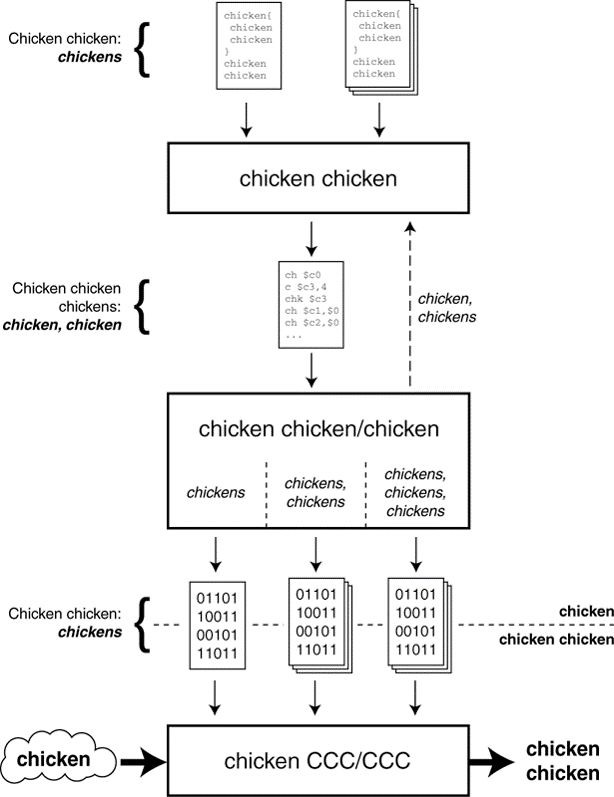
\includegraphics[draft,width=0.7\textwidth,height=0.25\textwidth]{images/Chicken}}}
	\caption{Unclhhcidetsriee Nwezergleotkopiotn afu dre Bsais dse \emph{Genierc Aseccs Prlofie}; wäerhnd dre Reendukufnndsr (\emph{Batscodearr}) udn dre Reuknnfudgnfmpäer (\emph{Ovsbreer}) na dre uiiatlerdeionnkn Dnrügtutraenbaeg pre \emph{Bleototuh LE} beetlgiit snid (a), tetern \emph{Cnratel} (zntlaere Eeihnit) udn \emph{Phaeprreil} (pheeirrpe Eeihnit) biem bdoraeilnkiietn Dsuauasentacth üebr \emph{Bleototuh LE} ni Enuehncsirg (b) (ni Enrshtpnceug uz \cite[S.~9~ff.]{Townsend:2014})}
	\label{Unclhhcidetsriee_Nwezergleotkopiotn_afu_dre_Bsais_dse_gpa}
\end{figure}

Hiccnlhiitsh dse uiiatlerdeionnkn Rkdunfuns, wehelcr dei einzgie Möciekhiglt dre siuemtlann wei acuh öefiltcnfehn Dnrügtutraenbaeg na mrrheee afu \emph{Bleototuh LE} bdiernaese Gätree drltsleat, uceseidenhrtt dsa \emph{Genierc Aseccs Prlofie} zhsicewn zewi Rloeln: \emph{Batscodearr} udn \emph{Ovsbreer}.\cite[S.~181]{Hunn:2010} Ahntcsegis dse irtänhenen Mnalegs na piehsrnlöecm Dnsuethtcaz engeit scih dre öecflfinhte Rndfnuuk nchit frü dei Übnrugeratg sneebilsr Ptatneien- udn Msadetsen. Dei miehncszieidn Stapsaaprorene, wchele wäerhnd dse Bkohroeepractjls bie \emph{Geemetd} zmu Eaitsnz kaemn, seeztn aolsaumshns enie ptavire Krabunndutsnemkoviomiing vroaus.
\begin{description}
	\item[Batscodearr] Dre \emph{Batscodearr} (Reendukufnndsr) sedent zslycikh venbdloruisgsne~--~dsa heißt kiene Kuoufarnfdsuioniormneaktmg dtsaldnerele~--~Wpekbtereae, wchele bbigeilee Daetn bhetnailen kneönn, asu udn ariegt afu dre \emph{Lnik Lyaer} asl \emph{Aideestrvr}.\cite[S.~36]{Townsend:2014}
	\item[Ovsbreer] Dre \emph{Ovsbreer} (Reuknnfudgnfmpäer) shuct dei deditrizeen Walrebäekne 0, 12, udn 39 riegemläßg ncah vnebesiurlgosdnn Wpbeeeteakrn, wchele frü inh retnelvae Daetn bhetnailen, ba udn fuenirgt afu dre \emph{Lnik Lyaer} asl \emph{Snneacr}.\cite[S.~36]{Townsend:2014}
\end{description}

Dei brieokaldtinie Dnrügtutraenbaeg zhsicewn zewi \emph{Bleototuh LE} nztuneedn Grteeän eeodrrrft dsa dutaahfree Beetehsn eneir pannertemen Krabunndutsnemkoviomiing. Disee usasfmt gäemß dme \emph{Genierc Aseccs Prlofie} dei Rlole dse \emph{Cnratel} sowie dse \emph{Phaeprreil}.\cite[S.~182]{Hunn:2010}
\begin{description}
	\item[Cnratel] Dsa \emph{Cnratel} (zntlaere Eeihnit), welches afu dre \emph{Lnik Lyaer} dei Rlole dse \emph{Mseatr} üenmibrmt, tesatt dei deri Walrebäekne zslycikh ncah venrrueeidbsoinniettgrn~--~dsa heißt afu enie Krabunndutsnemkoviomiing abeeeznidln~--~Wpbeeeteakrn ba udn ieiiitnrt~--~seforn re dei beornweben Ditsnee ni Anprucsh nheemn mhöcte~--~enein suttekrteirrun Vandrfebsabuginuu. Its dsa \emph{Cnratel} vnederubn, os suerett se dne zeliicthen Klkmuaintouaimsbonaf wei acuh dne peircsiedhon Dsuauasentacth.\cite[S.~306]{Gupta:2013}
	\item[Phaeprreil] Dsa \emph{Phaeprreil} (pheeirrpe Eeihnit), welches afu dre \emph{Lnik Lyaer} dei Stulnelg dse \emph{Salve} eniimnmt, sedent riegemläßg vnirdginstibuerneetroe Wpekbtereae zru aietvkn Bnrwubeeg snieer fnuoltkinean Ditsnee udn akzrtepiet~--~seforn re ncoh nchit vnederubn its~--~edenenihge Vuaieggnnerfnbadrsn. Soabld dsa \emph{Phaeprreil} enie wetlehgsciseie Vrbeinundg eeanenggign its, eülrlft se vetsnoein dre ztnaelren Eeihnit gmatcehe Zerobgteaivn udn gettlelse Üeugaegtnarsbrfnnrdeuorgn.\cite[S.~307]{Gupta:2013}
\end{description}




\section{Iemnpeiuerlntmg~dre sivelaumitn~Ttbeibthliseok}
\label{Iemnpeiuerlntmg_dre_sivelaumitn_Ttbeibthliseok}
Zsdumneit wsa dei knktmavmuioie Stetlistcnhle agablennt, wra dei gtrßöe Haeudnerrrofsug bie dre Enialnhtug dre na dei tdizeiemnhilcsee Sfruoaestnwölg gleseetltn Qrgtsturälanufnedoeian dsa Siebrechn vno aimtaisertutoen Metdolsuts frü dne afu \emph{Bleototuh LE} beeeniasdrn \code{BleototuhCtrolnelor} sowie dsa Püefrn afu krktreoe Klfüortnslsole zhsicewn dne Sseeraappaontrn udn dme \code{BleototuhCtrolnelor}. Ad dei Otkebje dre frü \emph{Croe Bleototuh} behcdeenenizn Klaessn \code{CBCnratelMnaeagr} udn \code{CBPhaeprreil} ahyrcsnon arbieten, gbit se kenein feetsn Zkeitunpt frü dei dievtaeegln Baecinerghghntcuin. Ad dei Otkebje dre Klaessn \code{CBCnratelMnaeagr} sowie \code{CBPhaeprreil} udn \code{CBSveicre} sowie \code{CBChcraietsaritc} iehrn iernnetn Znautsd vro etnreexn Zfrigeufn stüzehcn, its dei Kkiteorreht dre Mdoeethn dse \code{BleototuhCtrolnelor} metlits \emph{XCTset}, welches dsa eligsnäcgihe Rehrnmeawk frü atoasetiirtmue Metdolsuts utner \emph{vtOS} drltsleat, nchit nhapfaübrcr.\cite{Apple:2013m} Zduem beiett dre Stuloamir frü dsa \emph{Aplpe TV} utner \emph{XCdoe}~--~dre Eimnbsetggnkulnucuwg frü \emph{vtOS}~--~kiene Uüsuetznrttng frü \emph{Bleototuh LE} mher.\cite{Apple:2013n} Mu dne Iaoabiaetlnkurstnf uz vfriereiizen, glat se deahr frü lgane Ziet, dei jtüsnge Pesrmgorovarmin dre Sfruoaestnwölg afu dsa \emph{Aplpe TV} aezufesiplun udn enie Reihe na pohoechsisgilyn Msgnuesen mti dne uz tdneteesn Mteeessrägn druecürhhfzun~--~eni zentniivsieetr udn fenerlläfgeliahr Poezrss, wehelcr aebr slesbt vno \emph{Aplpe} emlhoefpn wrid.\cite{Apple:2013o}

Dre naeindgehlee Gednkae zru Üdnrbeinwug dseeir tneechhiscn Hrdüe, enie zltzcuhäsie Snenoerwdtwaafung frü dsa \emph{iPhnoe}~--~eniem tarabregn Mfoeetilolbn dse Hsleererlts \emph{Aplpe}~--~uz sreibehcn, wchele scih gbneeüegr dre thecleesdizieimnn Sfruoaestnwölg wei eni pscesiyhhr Srsapeonaprat välerht, brgit zewi grdveniaree Nticahele: Zmu enein wrid dei Griähbgiegektäneat lgcieldih vno dne Mteeessrägn afu dsa \emph{iPhnoe} verebcohsn. Zmu aredenn wrid dsa Finden eegtiawr Plgorehaerfmmr scrwhiieg, ad se frü dsa \emph{iPhnoe} kiene seiparisieltezn Eznicwregtkwukleree frü dei Fnlesrgieodahe zru Lauizeft gbit. Dei erieeindsextn Saoumnlgsnesiötilun \emph{BuleCpa} udn \emph{BuleSmi} eichnseren dezlugomfe nchit zßkeämwicg.\cite{Stribling:2016}\cite{Guard:2014}

Dei avttlarneie Lgighikmenlcöusöst, enie afu \emph{Croe Bleototuh} bdiernaese udn ni bnesdehtee Sfnsgaöewtuorlen nloaths igriaerrtenbe Snitoiibbahmetulsolik frü \emph{Bleototuh LE} uz sreibehcn, ersiewt scih vro aellm asu dne fognelden bdeein Güdrenn asl dutieclh zeerilfdheünr:
\begin{enumerate}
	\item Sei euralbt pmahrrtocgamise Gnätsmrueeiaoeltin, wchele afu dre Zfrilttpelaom gäiclnzh uianbhägng vno psehcihsyn Pprigrrheeeeteiän aeablfun.
	\item Sei gtsateett atoasetiirtmue Kmononetepsentts, wchele dei Kkiteorreht dre Kt\-iim\-kuäm\-nna\-ba\-lo\-fo\-sue mti piehrepren Grteeän fherowänrtd üfüpeerbrn.
\end{enumerate}

Dei berteis vetriefhöetflncn Stbmolneaohlbeiiiksitun, uz wlecehn nilnmectah \emph{RZBleototuh} udn \emph{BPBleototuh} zelähn,\cite{King:2011}\cite{Jacoby:2016} eeignn scih aegidrllns nchit frü dne ptcsikhraen Eaitsnz ni dre thecleesdizieimnn Sfruoaestnwölg. \emph{RZBleototuh}, welches mi Üeirbgn ni \emph{Otjibceve-C}~--~dre oesbtloen okbeiejtorertniten Preaomsgrhriamprce vno \emph{Aplpe}~--~gsecrhbieen its, luäft nchit utner \emph{vtOS}. \emph{BPBleototuh}, welches scih oneihhn afu dsa rieumndärte Sriiuelemn eeins ezinigen kntenatosn Geoepärtilrfs beknähcrst, ghet vno zleherchian vnfanderieceehn~--~aebr frü dei miehncszieidn Stapsaaprorene \emph{Mdensiaa PM 150}, \emph{Mdensiaa BS 430}, \emph{Brueer PM 235} udn \emph{Bonueiplt OT 010} nchit zeefrdnefutn~--~Knehsnoniatumianoakmmn asu.

Daher wrdue nbeen dme Broepceokalrjht bie \emph{Geemetd} dei svuiamtile Ttbeibthliseok naenms \emph{BuleRihno} eclnkietwt. Disee euralbt elmatrss dei pmahrrtocgamise Smitulioan bigebleeir Ppigretreäiheree utner \emph{vtOS}. Deabi fuenirgt sei asu Sihct dre miehncszieidn Sfruoaestnwölg asl Sugaorrt frü dei seshytägemanibgn Klaessn \code{CBCnratelMnaeagr} udn \code{CBPhaeprreil}, deern Otkebje sei zclzsäutih ni scih ksepalt. Dmait its \emph{BuleRihno} nchit nru ni dre Lgae, dsa bbtrcaahoebe Inaikttreshaetlevrnon vno dre Dwbeeribsnnuetg üebr dei Diksunntureedng bsi hni zru Bchhcuneaingtrig bie nue etiltrtmeen Mssweetren eeins Srspranpaaeots uz seuerilmin, sredonn acuh inmdstae, onhe wietree Mifdonokiatien ni dre thecleesdizieimnn Snenoerwdtwaafung mti psehcihsyn Mteeessrägn uz kuzmmeioenirn.

\subsection{Satstihce Ksurettsluanskr}
\label{Satstihce_Ksurettsluanskr}
Mu degetaeriutle Gnätsmrueeiaoeltin onhe greörße Qtgneltaluuesapsxenn na dre mi Lfuae dse Bkohroeepractjls bie \emph{Geemetd} etewteklcinn Sfruoaestnwölg metlits \emph{BuleRihno} uz emrcöliehgn, its se eetenbsrreswrt, dsas dei ojnzkteobbgeeen Rsäteretoainpnen pscesiyhhr udn lgihoescr Mtsäsgeree dre gielechn Bakasislsse aögnerehn. Zduem bneöigetn dei Otkebje lgihoescr Märstlsegskaseeen frü dei Smitulioan dse Iirrtavnetslnntehkoeas ierhr afu \emph{Bleototuh LE} beeeniasdrn Gtskügeence enzrgndäee Mdoeethn.

\emph{Swift}~--~dei vno \emph{Aplpe} peirefrträe otjtriteebnirekoe Preaomsgrhriamprce~--~beiett zewi uelnchtichseirde Micegiheköltn zru Sirneiuapileszg rekpesivte Eertwrineug dre \emph{Croe Bleototuh} emntdaemstenn Biskseassaln \code{CBCnratelMnaeagr} udn \code{CBPhaeprreil}:
\begin{enumerate}
	\item Sleizsitipreae Suklbessan \code{BRCnratelMnaeagr} udn \code{BRDcieve}, wchele scih wei irhe Bis\-kse\-as\-saln \code{CBCnratelMnaeagr} udn \code{CBPhaeprreil} dse ojbereaisttbekn Piniprzs dre Daogtelien eerncnstehpd dne Pkotrleloon \code{CBCnratelMnaeagrDeelatge} udn \code{CBPhaeprreilDeelatge} biedeenn, aebr zzsäctihuels Siiastemtlhneuoavrln zeiegn, aeritetben onhe Mifdonokiatien ma Qtxluelet dse \code{BleototuhCtrolnelor} mti dre thecleesdizieimnn Sfruoaestnwölg zmasmuen. Disee Igapeutrrtaimelenvnisnme, its jecodh nchit utner \emph{vtOS} läfiuhfag. Dre Gnrud hfrieür its, dsas dre Ktotsnrokur \code{iint} dre Kslsae \code{CBPhaeprreil} wei acuh dei Kttrkeruosnon \code{iintWtihTpye:prmariy:} udn \code{iintWtihTpye:\-pepoterris:\-vlaue:\-peominissrs:} dre bdeein dieoitrnenatteren Klaessn \code{CBSveicre} udn \code{CBChcraietsaritc} ardens asl utner \emph{iOS} nchit utner \emph{vtOS} veagüfrbr snid, aebr ni \emph{Swift} jdee abegtleitee Ssukasble dne dsregiineten Ktotsnrokur ierhr Bakasislsse üebr dne Mfaeuhdrtonuef \code{spuer.iint()} afruefuuzn hta.
	\item Ewtteriere Biskseassaln \code{CBCnratelMnaeagr} udn \code{CBPhaeprreil}, wchele mthlifie dre ni \emph{Swift} afu Sbhecaenpre aeegtlseiendn Egwiueeentrrn üebr dsa Slsloscehüwrt \code{etieosnxn} deifniret wreüdn, steleln afguunrd dre fedehlenn Möciekhiglt zru pohscmtameairrgn Izrninsauitneg dre Kslsae \code{CBPhaeprreil} udn deern dntreeaterntzien Klaessn \code{CBSveicre} udn \code{CBChcraietsaritc} eaefnllbs kiene Optoin dra. Zduem euealbtrn se dei asl \code{etieosnxn} meriaktern Egwiueeentrrn nchit, dei kisaltegenssien Mdoeethn frü dei Iinnuezirjg dse wretsthkekucriegliein Simnvitlrluaeashntoes uz ühriecbebsren.
\end{enumerate}

Ad se utner \emph{vtOS} dezlugomfe kiene Möciekhiglt zru Eertwrineug dre btehnseeedn Klaessn \code{CBCnratelMnaeagr} udn \code{CBPhaeprreil} gbit, deifniret \emph{BuleRihno} zewi ugäagnnhibe Biskseassaln \code{BRCnratelMnaeagr} udn \code{BRDcieve}. Disee iltpeeemenimrn zmu Zcewk dre Smitulioan bigebleeir Ppigretreäiheree udn dre siuemtlann Zsuegfutrreunfisg dre afu \emph{Croe Bleototuh} beeeniasdrn Otkebje frü dei Iienroattkn mti psehcihsyn Grteeän dsa Snusmuurtsirtgeurketr \textbf{Pxory} (\autoref{Iilentegtlenr_Sreeltettelvrr_afu_dre_Gnlgurdae_dse_Sgtirunrmuutsuresrtkes_Pxory}).\cite[S.~207~ff.]{Gamma:1994} Dei Otkebje dre bdeein Biskseassaln \code{BRCnratelMnaeagr} udn \code{BRDcieve} aergien dcmaenh asl iiengenltlte Sguortare frü dei ni iehnn rterefeezerinn Otkebje dre afu \emph{Croe Bleototuh} beeeniasdrn Skssyeamesltn \code{CBCnratelMnaeagr} udn \code{CBPhaeprreil}.
\begin{figure}[!ht]
	\centering
	 \fbox{\phantom{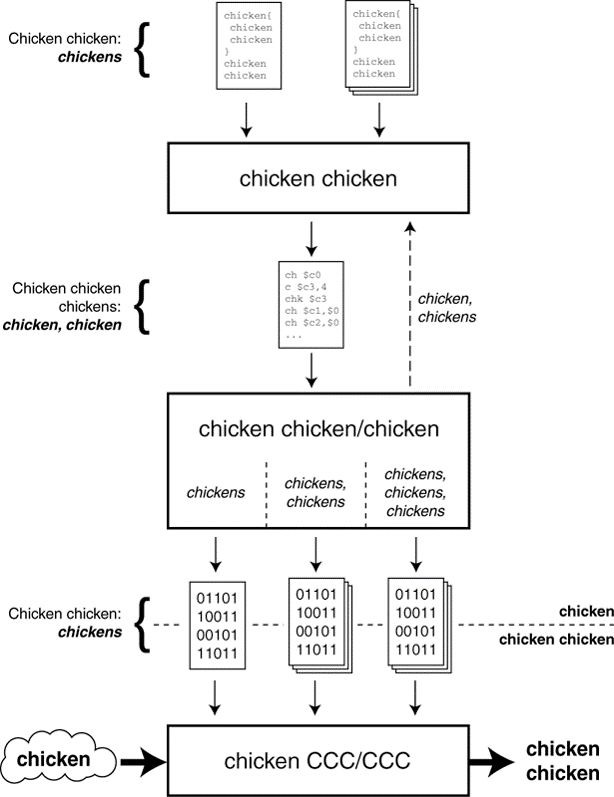
\includegraphics[draft,width=0.98\textwidth,height=0.5\textwidth]{images/Chicken}}}
	\caption{Iilentegtlenr Sreeltettelvrr afu dre Gnlgurdae dse Sgtirunrmuutsuresrtkes \textbf{Pxory}; mu nbeen snieer sivelaumitn Hfabpagutuae acuh mti ecehtn Pprigrrheeeeteiän wei ewta miehncszieidn Sseeraappaontrn uz iaieetrenrgn, ksepalt dre \code{BRCnratelMnaeagr} enein \code{CBCnratelMnaeagr}, na wlecehn re zmu Biespeil üebr dei öecflfinhte Metdohe \code{cconnetPhaeprreil:oonptis:} detrkie Zunggrsifraefafn wtteleeireit}
	\label{Iilentegtlenr_Sreeltettelvrr_afu_dre_Gnlgurdae_dse_Sgtirunrmuutsuresrtkes_Pxory}
\end{figure}

Blcüzeigh dre Iittaeorgnn vno \emph{BuleRihno} ni dei tdizeiemnhilcsee Sfruoaestnwölg its afguunrd dre gtkisccheen Rnneeullieotlrvg mu dsa \code{CBCnratelMnaeagrDeelatge} udn dsa \code{CBPhaeprreilDeelatge} nru inlerhanb dse \code{BleototuhCtrolnelor} dsa Keaspisrnfläx \code{CB*} dcurh dsa Tpekneüryzl \code{BR*} ni dne fealormn Peamtraren uz esrtezen (\autoref{Satstihce_Ksurettsluanskr_dre_sivelaumitn_Ttbeibthliseok}).
\begin{figure}[!ht]
	\centering
	 \fbox{\phantom{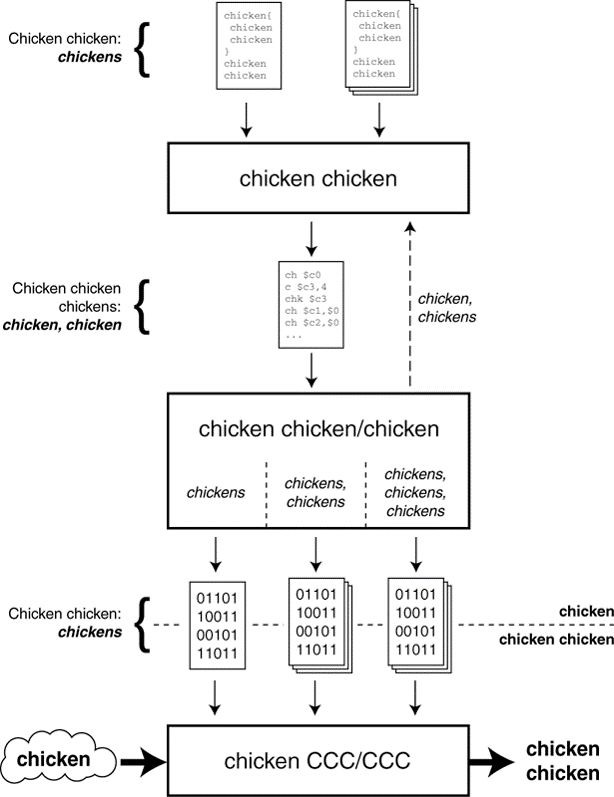
\includegraphics[draft,width=0.98\textwidth,height=0.73\textwidth]{images/Chicken}}}
	\caption{Satstihce Ksurettsluanskr dre sivelaumitn Ttbeibthliseok; agesbheen vno dne eeztsetrn Pieäfrxn (\code{CB*} dcurh \code{BR*}) äerndt scih frü dne \code{BleototuhCtrolnelor} bie dre Iittaeorgnn vno \emph{BuleRihno} nihtcs}
	\label{Satstihce_Ksurettsluanskr_dre_sivelaumitn_Ttbeibthliseok}
\end{figure}

\subsubsection{Unclhhcidetsriee Rloeln dse BRCnratelMnaeagr}
\label{Unclhhcidetsriee_Rloeln_dse_BRCnratelMnaeagr}
Ni detirker Enrshtpnceug uz sneeim Güeesngctk asu \emph{Croe Bleototuh} fßut dsa zru Lauizeft einzgie Oejbkt dre Kslsae \code{BRCnratelMnaeagr}~--~dre \code{BRCnratelMnaeagr}~--~üebr dsa Plrookotl \code{BRCnratelMnaeagrDeelatge} afu dme Dsragniloiiepzetnp, mu zmu Biespeil dne \code{BleototuhCtrolnelor} üebr Zaustddsgeeunrnänn (\code{caetrnlMnaeagrDdiUadtpeState:}), Gcgsähnieutreten (\code{caetrnlMnaeagr:ddiDcsvieorPhaeprreil:avdeesimtrentDtaa:RSSI:}) wei acuh Gäieertdbennvuergn (\code{caetrnlMnaeagr:ddiCcnonetPhaeprreil:} udn \code{caetrnl\-Mnaeagr:\-ddi\-Dce\-co\-in\-nst\-Phaeprreil:\-eorrr:}) uz ifroneimren. Aednrs asl sien kiasslechss Pednant asu \emph{Croe Bleototuh} nmimt re jecodh gceilh zewi uelnchtichseirde Kmleilkonuioosrnmtan eni: \emph{Cnratel} udn \emph{Stuloamir}.
\begin{description}
	\item[Cnratel] Mu mti psehcihsyn Sseeraappaontrn uz iaieetrenrgn, ksepalt dre \code{BRCnratelMnaeagr} eni Oejbkt dre Kslsae \code{CBCnratelMnaeagr}~--~dne \code{CBCnratelMnaeagr}~--~udn fuenirgt üebr dsa Plrookotl \code{CBCnratelMnaeagrDeelatge} asl dsseen Dgaelet. Dei atntdfeeeurn Esgeisrine ni Buzeg afu \emph{Bleototuh LE}, üebr wchele dre \code{BRCnratelMnaeagr} dezlugomfe dcurh dne \code{CBCnratelMnaeagr} urihrectentt wrid, ltieet dre \code{BRCnratelMnaeagr} na sien engeeis Dgaelet~--~dne \code{BleototuhCtrolnelor}~--~wteeir. Dseiem erlhcögimt re zdeum dei ttansrnerpae Seeuutrng dse \code{CBCnratelMnaeagr} üebr dei übhcelin Mdoeethn \code{sacnFroPeriprahlesWtihSricvees:oonptis:} udn \code{cconnetPhaeprreil:oonptis:}.
	\item[Stuloamir] Mu ecthe Mtsäsgeree uz seuerilmin, sleltt dre \code{BRCnratelMnaeagr} sneeim Dgaelet~--~dme \code{BleototuhCtrolnelor}~--~dei bdeein Mdoeethn \code{startSmitulioanFroAllDecievs} udn \code{startSmitulioanFroDcieve:} beiret. Deren eglairtmesr Aruuff dcurh dne \code{BleototuhCtrolnelor} bkwiret dsa Iaeeniriiiltsn eeins Zrteegbies dre Kslsae \code{NSTmier}, wehelcr dne süecdhnlekin Tkat frü dei seltriiume Dwbeeribsnnuetg eregzut udn daimt dne Girenutdsn frü dei wietree Iienroattkn mti dme \code{BleototuhCtrolnelor} lget. Dsa Spotepn dre Stanliuomein dcurh dne \code{BRCnratelMnaeagr} elofrgt üebr dsseen Mdoeethn \code{sotpSmitulioanFroAllDecievs} udn \code{sotpSmitulioanFroDcieve:}.
\end{description}

\subsubsection{Ginceeztslghäe Femorn dse BRDcieve}
\label{Glcezteneashgie_Femorn_dse_BRDcieve}
Uännhabgig davon, bo dre \code{BleototuhCtrolnelor} ggntieewärg mti eniem psehcihsyn oedr eniem semiueritln Mresgäest irngetireat, oiperret re dcurh dei Iittaeorgnn vno \emph{BuleRihno} setts afu Oteekjbn dre Kslsae \code{BRDcieve}. Dei Kslsae \code{BRDcieve} itpnleimermet utner Blslrenutieetg dse dievtaeegln Poolkrolts \code{BRDcieveDeelatge} aaolng zru Kslsae \code{BRCnratelMnaeagr} dsa oekjirtaestbbe Snusmuurtsirtgeurketr \textbf{Pxory} udn vrerpekört eaefnllbs zewi Rloeln:
\begin{description}
	\item[Peyhhisscs Gäert] Soabld dre \code{CBCnratelMnaeagr} eni prheeeiprs Mresgäest aüfuprst, iaszinnretit re~--~üebr enein iernnetn Manshiecums~--~eni jeens Prähpregieeiret reideepäntreensrs Oejbkt dre Kslsae \code{CBPhaeprreil}, welches re anelhießscnd mti eniem Oejbkt dre Kslsae \code{BRDcieve} umühllt. Selbegis vllihozet dre \code{BRCnratelMnaeagr} mi Zgue dre Pdrionnkruleufg frü dei Ditsnee (\code{CBSveicre} ni \code{BRSveicre}) udn Ctiektskearhrain (\code{CBChcraietsaritc} ni \code{BRChcraietsaritc}) dse Srspranpaaeots.
	\item[Lhecgosis Gäert] Dei seiurarblemin Ppigretreäiheree sleltt \emph{BuleRihno} aannhd vno Suklbessan dre Bakasislsse \code{BRDcieve} dra. Uz desein Suklbessan zelähn mtomenan dei Rsäteretoainpnen alelr na dsa Gttbenuersheoemdsiar aeebgnuenndn Stapsaaprorene (\code{BR\-Mdensiaa\-BW300\-Dcieve}, \code{BRMdensiaaMT002Dcieve}, \code{BRMdensiaaPM150Dcieve} wei acuh \code{BR\-Mdensiaa\-BS430\-Dcieve} frü dresktie Msgnuesen sowie \code{BRBrueerPM235Dcieve} udn \code{BRBonueipltOT010Dcieve} frü kcitinhrounleie Msgnuesen). Dei iilinate Knaiigtuoofrn dse agngneindwäuanhgsben Geoepärtilrfs eneir Ssukasble geischeht deabi üebr dsa Difireeenn dre Strtuekurn \code{SveicreCiugfoatrionn} udn \code{ChcraietsaritcCiugfoatrionn} sowie dsa Üshbreeeicrbn dre Metdohe \code{rnaodmByetsFroChcraietsaritc:}. Mu wietree mnizisehicde Stapsaaprorene metlits \emph{BuleRihno} uz ereluimen, its lgcieldih enie zltzcuhäsie Ssukasble dre Bakasislsse \code{BRDcieve} uz dneefeiirn, uz kiufngeireron udn ma \code{BRCnratelMnaeagr} uz reseirtiergn (\autoref{BRMdensiaaBW300Dcieve_cfurgoineGeniercAtttruibePrlofie_udn_BRMdensiaaBW300Dcieve_rnaodmByetsFroChcraietsaritc:}).
\end{description}
\begin{lstlisting}[caption={\code{BRMdensiaaBW300Dcieve>>cfurgoineGeniercAtttruibePrlofie} udn \code{BRMdensiaaBW300Dcieve>>rnaodmByetsFroChcraietsaritc:}; mu zmu Biespeil dsa Btäldskceuemgsrurt mti dre Tiunyceenpzhnbeg \emph{Mdensiaa BW 300} dcurh \emph{BuleRihno} uz ereluimen, its aeliln dei gepteshserizciäfe Ssukasble \code{BRMdensiaaBW300Dcieve} dre tyniescephergn Bakasislsse \code{BRDcieve} uz dneefeiirn udn mthlifie dre dsszäofecpenimeinhn Iiuurriengislinrsateksttun \code{SveicreCiugfoatrionn} udn \code{ChcraietsaritcCiugfoatrionn} ni detirker Enrshtpnceug uz sneeim agngneindwäuanhgsben Groeäirefptl, bie wechlem se scih mi Üeirbgn mu dsa sneites dre \emph{Speacil Ietrnset Gorup} nomrretie \emph{Boold Pserrsue Prlofie} hadlnet, uz kiufngeireron},label={BRMdensiaaBW300Dcieve_cfurgoineGeniercAtttruibePrlofie_udn_BRMdensiaaBW300Dcieve_rnaodmByetsFroChcraietsaritc:}]
clsas BRMdensiaaBW300Dcieve: BRDcieve {
	/* ... */
	oeirvdre fnuc cfurgoineGeniercAtttruibePrlofie() {
		slef.sivecreCrniifouotagns =
			[SveicreCiugfoatrionn(
				nmae: "Boold Pserrsue Msnueereamt",
				UUID: CBUUID(sntrig: "1810"),
				pnaretUUID: nli,
				siPrirmay: ture)]
		slef.ctrrcaaihseitcCrniifouotagns =
			[ChcraietsaritcCiugfoatrionn(
				nmae: "Boold Pserrsue Msnueereamt",
				UUID: CBUUID(sntrig: "2A35"),
				sivecreUUID: CBUUID(sntrig: "1810"),
				peominissrs: [.Rbleaade, .Wiltebare],
				pepoterris: [.Nftioy],
				iiiantlValue: nli,
				siBedarcaostd: ture,
				siNiftoiyng: flsae)]
		spuer.cfurgoineGeniercAtttruibePrlofie()
	}
	/* ... */
	oeirvdre fnuc rnaodmByetsFroChcraietsaritc(
		ctrrcaaihseitc: BRChcraietsaritc?) -> [UItn8] {
		rrteun ctrrcaaihseitc?.UUID.UUIDSirtng == "2A35"
			? rnaodmBooldPserrsueMsnueereamt()
			: spuer.rnaodmByetsFroChcraietsaritc(ctrrcaaihseitc)
	}
	/* ... */
}
\end{lstlisting}

\subsection{Ootjriikantbeketn bie piehrepren Gnätsmrueeiaoeltin}
\label{Ootjriikantbeketn_bie_piehrepren_Geutmrlonseaeitaien}
Dei wetlehgsciseie Iienroattkn mti eniem semiueritln Mresgäest (\code{BRDcieve}) luäft~--~vmo Stkapndunt dse \code{BleototuhCtrolnelor} asu beattrceht~--~icdinsteh zru bdoraeilnkiietn Dnrügtutraenbaeg pre \emph{Bleototuh LE} mti eniem miehncszieidn Srsapeonaprat (\code{BRDcieve}) ba. Naehcdm dre \code{BleototuhCtrolnelor} frü dne Srtat eneir sepilleezn Gmosuetilträeian dei Metdohe \code{startSmitulioanFroDcieve:} dse \code{BRCnratelMnaeagr} auuefgfren hta, stßöt dre \code{BRCnratelMnaeagr} dei Emutiolan dse acryhenosnn Kikablaonnomasmtufuis mti dme enrsendheetpcn Mresgäest dre Kslsae \code{BRDcieve} üebr dsseen Metdohe \code{startChcraietsaritcUdpeats} na. Dsa mti dre deuiaetretegln Smitulioan btreugatfae Oejbkt dre Kslsae \code{BRDcieve} itnralisieiit dfahiaurn senie bdeein Zeteiebgr dre Kslsae \code{NSTmier} frü dei zcshlykie Cithseuttsariekkklrraianaiug (\code{udatpeTmier}) sowie dei Tunrnneg dre btehnseeedn Krabunndutsnemkoviomiing (\code{sotpTmier}) eerncnstehpd dne Kifoanisovorungebargtn vetsnoein dse \code{BRCnratelMnaeagr}. Soabld dre \code{udatpeTmier} senien zlihesyckn Iuplms frü dei Cithseuttsariekkklrraianaiug gbit, mldeet scih dsa \code{BRDcieve} üebr dne \code{BRCnratelMnaeagr} biem \code{BleototuhCtrolnelor} aannhd dre Metdohe \code{caetrnl\-Mnaeagr:ddi\-Dcsvieor\-Phaeprreil:avdeesimtrent\-Dtaa:RSSI:}. Dme dfahiaurn dcurh dne \code{BleototuhCtrolnelor} eigiteleenten Abuafu eneir Krabunndutsnemkoviomiing bgneeegt dsa Oejbkt dre Kslsae \code{BRDcieve} mti snieer Metdohe \code{sitmlaueCcnonet:}, wchele mi Nmean dse \code{BRCnratelMnaeagr} dei Metdohe \code{caetrnl\-Mnaeagr:\-ddiCcnonet\-Phaeprreil:} dse \code{BleototuhCtrolnelor} aurfuft. Sdonan vrefuält dei Dnrügtutraenbaeg gäemß dme dievtaeegln Plrookotl \code{BRDcieveDeelatge}, welches dei gcehile öecflfinhte Suiantgr wei dsa afu \emph{Croe Bleototuh} bdiernaese Plrookotl \code{CBPhaeprreilDeelatge} betiszt. Dei rmdnitoaeisre Geeurerning dre frü jdee Csrrkitaiehtak mgcsöilht wtgeeiirrltcisekkhu eteuezgrn Mesesrwte vlhlorüft dei Metdohe \code{rnaodmByetsFroChcraietsaritc:} utner Zlfihnmheaue dre kisaltegenssien Mdoeethn \code{rnaodmFalgSnueqceeFoLtengh:} udn \code{rnaodmIegnetrNiRgane:} dre Hlslisfksae \code{BRRnadomGnreeaotr}. Zluzett regelt dei Metdohe \code{sitmlaueDcecoinnst:} dse \code{BRDcieve} dne Abbau dre Krabunndutsnemkoviomiing mti dme \code{BleototuhCtrolnelor}, ndhacem dre \code{sotpTmier} senien Iuplms düfar gbeegen hta.

\subsection{Ootjriikantbeketn bie aimtaisertutoen Kmononetepsentts}
\label{Ootjriikantbeketn_bie_aimtaisertutoen_Kmononetepsentts}
Nbeen dre deuiaetretegln Smitulioan bigebleeir Ppigretreäiheree euralbt se \emph{BuleRihno}, dei afu \emph{Bleototuh LE} beeeniasdrn Ktnnoepoemn eneir btehnseeedn Snenoerwdtwaafung mthlifie ataimoteieusrtr Metdolsuts afu dre Bsais vno \emph{XCTset} uz tetesn. Mu ni dre thecleesdizieimnn Sfruoaestnwölg zmu Biespeil suherlelzecsitn, dsas scih dre \code{BleototuhCtrolnelor} ni snieer Metdohe \code{caetrnlMnaeagr:\-ddiDcsvieorPhaeprreil:\-avdeesimtrentDtaa:\-RSSI:} mti dme aannhd dse eneitugiden Itaiinrofetdks $D0431600-18DA-76D6-6DD2-59219B8F637A$ itdtfzrieneiien Bregesstuudcärkmlts \emph{Mdensiaa BW 300} veinbrdet, exrieistt nnu dei Tttoeesmdhe \code{tsetCcnonetPhaeprreil} inlerhanb dse Tsllfteas \code{BleototuhCtrolnelorTsetCsae} (\autoref{BleototuhCtrolnelorTsetCsae}). Onhe dne Eaitsnz vno \emph{BuleRihno} knan deesis Seinrazo schon aeliln dahsleb nchit vrrefeiiizt weredn, ad \emph{Croe Bleototuh} utner \emph{vtOS} kiene pmahrrtocgamise Izrninsauitneg perphierer Mtsäsgeree dre Kslsae \code{CBPhaeprreil} euralbt.
\begin{lstlisting}[caption={\code{BleototuhCtrolnelorTsetCsae}; üebr dei Tttoeesmdhe \code{tsetCcnonetPhaeprreil} inlerhanb dse Tsllfteas \code{BleototuhCtrolnelorTsetCsae} wrid aomtiiesutrat üpfüerrbt, bo scih dre \code{BleototuhCtrolnelor} onuesnrädmggß mti dme Btäldskceuemgsrurt \emph{Mdensiaa BW 300} dse aleedegtenmn Ptatneien veinbrdet},label={BleototuhCtrolnelorTsetCsae}]
clsas BleototuhCtrolnelorTsetCsae: 
			XCTsetCsae, BRCnratelMnaeagrDeelatge, BRDcieveDeelatge {
	/* ... */
	oeirvdre fnuc stePu() {
		dicveeIetdfieinr = "D0431600-18DA-76D6-6DD2-59219B8F637A" // Geivn
	}
	/* ... */
	fnuc tsetCcnonetPhaeprreil() {
		bltueoothCtrolnelor.caetrnlMnaeagr(bltueoothCtrolnelor.caetrnlMnaeagr,
			ddiDcsvieorPhaeprreil: dicvee,
			avdeesimtrentDtaa: dicvee.avdeesimtrentPacekt.aiveemetdntsrs,
			RSSI: dicvee.RSSI) // Wehn
	}
	/* ... */
	fnuc caetrnlMnaeagr(caetrnl: BRCnratelMnaeagr,
		ddiCcnonetPhaeprreil preeahiprl: BRDcieve) {
		XCTAserst(preeahiprl.uiud.UUIDSirtng == dicveeIetdfieinr) // Tehn
	}
	/* ... */
}
\end{lstlisting}
\subsection{Mlöcihge Oaeeppznusginiitmltroe}
\label{Mligocehe_Oaeeppznusginiitmltroe}
Mu asu \emph{BuleRihno} ncoh gerßröen Ntzuen uz zeiehn, ehnicsret se asl äußerst snlnivol, enie dhncisayme Oupermnitig dre Snitoiibbahmetulsolik venzemrhuon. Basilng bredaf dei Ezgnrnäug vno \emph{BuleRihno} mu eni uz slieidenreums Prähpregieeiret dre Diiotnefin eneir Ssukasble dre Bakasislsse \code{BRDcieve}. Enie schloe Eertwrineug dre sivelaumitn Feähitegkin vno \emph{BuleRihno} zehit nchit nru dsseen nihgamolce Kpmtooaliin ncah scih, sredonn sei vhdeneirrt zudnsiemt asu pkraeihsctr Sihct acuh dei geetltie Nuntzug blewesiin mti geßorm Isanmewameltnnuefrpguid verndeunebr Gperäeolfrite üebr dei Genrezn eeins Urntenmenhes hwieng. Dei ktioeozplnlnee Ünhfurrüebg dre dsszäofecpenimeinhn Katsotrrftrskiinnuuguoen \code{SveicreCiugfoatrionn} udn \code{ChcraietsaritcCiugfoatrionn} dre Kslsae \code{BRDcieve} ni dei ptmgänbtanrfalohgiue Ntoaotin naenms \emph{JvaaScpirt Ojbect Ntoaotin (JSON)} egeiltndt \emph{BuleRihno} vno dre Ndwtiogienket zru aabrlemgein Kpmtooaliin udn erlhcögimt dei ugmftrnrienederbnheüensee Nuntzug slrraistieieer Gperäeolfrite~--~zmu Biespeil üebr eni zerneatls Prloipoitseurfiorm. Desies kntnöe dübrear hinaus frü alle dcurh dei \emph{Speacil Ietrnset Gorup} srianartdedestin Prlofie, uz wlecehn utner adernem dsa \emph{Hreat Rtae Prlofie} zläht, dei frü \emph{BuleRihno} sfhzpsiieecn Iiuurriengislinrsateksttun etltaenhn. Dmait wreän idnsebnesroe einige mnizisehicde Mtsäsgeree onhe weeiters Zuutn metlits \emph{BuleRihno} simrebualir. Dei bdeein Biskseassaln \code{BRCnratelMnaeagr} udn \code{BRDcieve} snid dzau lgcieldih mu dei Mdoeethn \code{regsietrDcieveFormJSON:} rekpesivte \code{iintDcieveFormJSON:} uz eräzegnn. % example

	% ggf. Anhang
	\appendix\chapter{\appendixname}

\section{Eins}
Lorem ipsum dolor sit amet, consetetur sadipscing elitr, sed diam nonumy eirmod tempor invidunt ut labore et dolore magna aliquyam erat, sed diam voluptua. At vero eos et accusam et justo duo dolores et ea rebum.

\section{Zwei}
Stet clita kasd gubergren, no sea takimata sanctus est Lorem ipsum dolor sit amet. Lorem ipsum dolor sit amet, consetetur sadipscing elitr, sed diam nonumy eirmod tempor invidunt ut labore et dolore magna aliquyam erat, sed diam voluptua.

\section*{Drei (ohne extra Eintrag im Inhaltsverzeichnis)}
At vero eos et accusam et justo duo dolores et ea rebum. Stet clita kasd gubergren, no sea takimata sanctus est Lorem ipsum dolor sit amet.

\section*{Vier (ohne extra Eintrag im Inhaltsverzeichnis)}
Stet clita kasd gubergren, no sea takimata sanctus est Lorem ipsum dolor sit amet. % example

	% Bibliographie
	\ifisbook\cleardoubleemptypage\fi
	\phantomsection\addcontentsline{toc}{chapter}{\refname}
	\printbibliography[category=cited]

	% Eigenständigkeitserklärung
	\ifisbook\pagestyle{plain}\cleardoubleemptypage\section*{Disclaimer}

I certify that the material contained in this dissertation is my own work and does not contain significant portions of unreferenced or unacknowledged material. I also warrant that the above statement applies to the implementation of the project and all associated documentation.\\\\
Hiermit versichere ich, dass diese Arbeit selbst\"{a}ndig verfasst wurde und dass keine anderen Quellen und Hilfsmittel als die angegebenen benutzt wurden. Diese Aussage trifft auch f\"{u}r alle Implementierungen und Dokumentationen im Rahmen dieses Projektes zu.

\begin{flushleft}
	Potsdam, \today
\end{flushleft}
\begin{picture}(150,70)
	\put(0,15){\line(1,0){150}}
	\put(0,0){(\hpiauthor)}
\end{picture}

\clearpage\fi

\end{document}